\chapter{Le m\'etier d'enseignant\mp e-chercheur\mp euse}


%%%%%%%%%%%%%%%%%%%%%%%%%%%%%%%%%%%%%%%%%
\section{Attributions et environnement}
La cat\'egorie des enseignant\mp e\mp s-chercheur\mp euse\mp s (EC) comprend 2 corps distincts :
les ma\^\i tres de conf\'erences (MCF) et les professeur\mp e\mp s des universit\'es (PR).

Les \textbf{ma\^\i  tres de conf\'erences} sont des fonctionnaires titulaires
nomm\'e\mp e\mp s sur un emploi dans un \'etablissement public d'enseignement
sup\'erieur et de recherche par arr\^et\'e minist\'eriel. 
%La fiche m\'etier du minist\`ere est disponible \`a l'adresse :

Les MCF sont nomm\'e\mp e\mp s en qualit\'e de stagiaire pour une dur\'ee d'un an par arr\^ et\'e du ministre charg\'e de l'enseignement sup\'erieur.
A l'issue du stage pr\'evu, les MCF stagiaires sont soit titularis\'e\mp e\mp s, soit maintenu\mp e\mp s en qualit\'e de stagiaires pour une p\'eriode d'un an, soit r\'eint\'egr\'e\mp e\mp s dans leur corps d'origine, soit licenci\'e\mp e\mp s s'ils ou elles n'ont pas la qualit\'e de fonctionnaire. Les d\'ecisions sont prononc\'ees par arr\^ et\'e du ou de la pr\'esident\mp e ou du ou de la directeur\mp rice de l'\'etablissement conform\'ement \`a l'avis, selon le cas, de la Commission de la recherche de l'\'etablissement ou de l'organe en tenant lieu, ou, s'il a \'et\'e saisi, du Conseil d'administration, instances si\'egeant, dans tous les cas, en formation restreinte aux enseignant\mp e\mp s-chercheur\mp euse\mp s et chercheur\mp euse\mp s (ou assimil\'e\mp e\mp s).

\textbf{Lien utile\hspace{.5em}}\url{https://www.enseignementsup-recherche.gouv.fr/fr/maitres-de-conferences-46317}

Les \textbf{professeur\mp e\mp s des universit\'es} sont des fonctionnaires titulaires nomm\'e\mp e\mp s sur un emploi dans un \'etablissement public d'enseignement
sup\'erieur et de recherche par d\'ecret de la P\'esident\mp e de la R\'epublique. 
%La fiche m\'etier du minist\`ere est disponible \`a l'adresse : \url{https://www.enseignementsup-recherche.gouv.fr/fr/professeur-des-universites-46367}.

\textbf{Lien utile\hspace{.5em}}\url{https://www.enseignementsup-recherche.gouv.fr/fr/professeur-des-universites-46367}
 
Les EC concourent \`a l'accomplissement des missions de service
public de l'enseignement sup\'erieur. Ils et elles participent \`a
l'\'elaboration et \`a la transmission des connaissances, assurent
la direction, le conseil et l'orientation des \'etudiants. Elles et ils
contribuent \'egalement au d\'eveloppement de la recherche
fondamentale et appliqu\'ee, \`a sa valorisation, ainsi qu'\`a la
diffusion de la culture et \`a la coop\'eration internationale. Ils et elles
assurent en outre des t\^aches relatives \`a l'administration et \`a
la gestion de leur \'etablissement de rattachement. Les PR ont g\'en\'eralement pour responsabilit\'e suppl\'ementaire, par
rapport aux MCF, d'encadrer les \'equipes de
recherche, d'assurer la direction des UFR, des laboratoires.

\index{Enseignant\mp e-chercheur\mp euse (EC)}
\index{Ma\^\i tre\mp sse de conf\'erences (MCF)}
\index{Professeur\mp e des universit\'es (PR)}

En 2021, il y avait 3045 EC dans les sections 25 et 26 du Conseil National des Universit\'es (CNU, \textit{c.f.}, Chapitre \ref{CNU}), soit 6,36\% des effectifs totaux des sections CNU, et dont environ 2 tiers sont MCF (\textit{c.f.}, Figure \ref{fig.cnu}). Entre 2013 et 2021 la proportion de femmes en math\'ematiques a augment\'e de presque 2 points passant de 20,5\% \`a 22,1\% au niveau national. On peut n\'eanmoins observer une disparit\'e importante entre les sections 25 (13,8\% de femmes) et 26 (28,5\% de femmes). Il existe \'egalement un d\'es\'equilibre important chez les PR (13,5\% de femmes) et les MCF (27,5\% de femmes).

\begin{figure}[t]
\subfloat[\'Evolution du nombre d'enseignant\mp e\mp s-chercheur\mp euse\mp s des sections 25 et 26 du CNU]{
\label{fig.cnu.demo}%
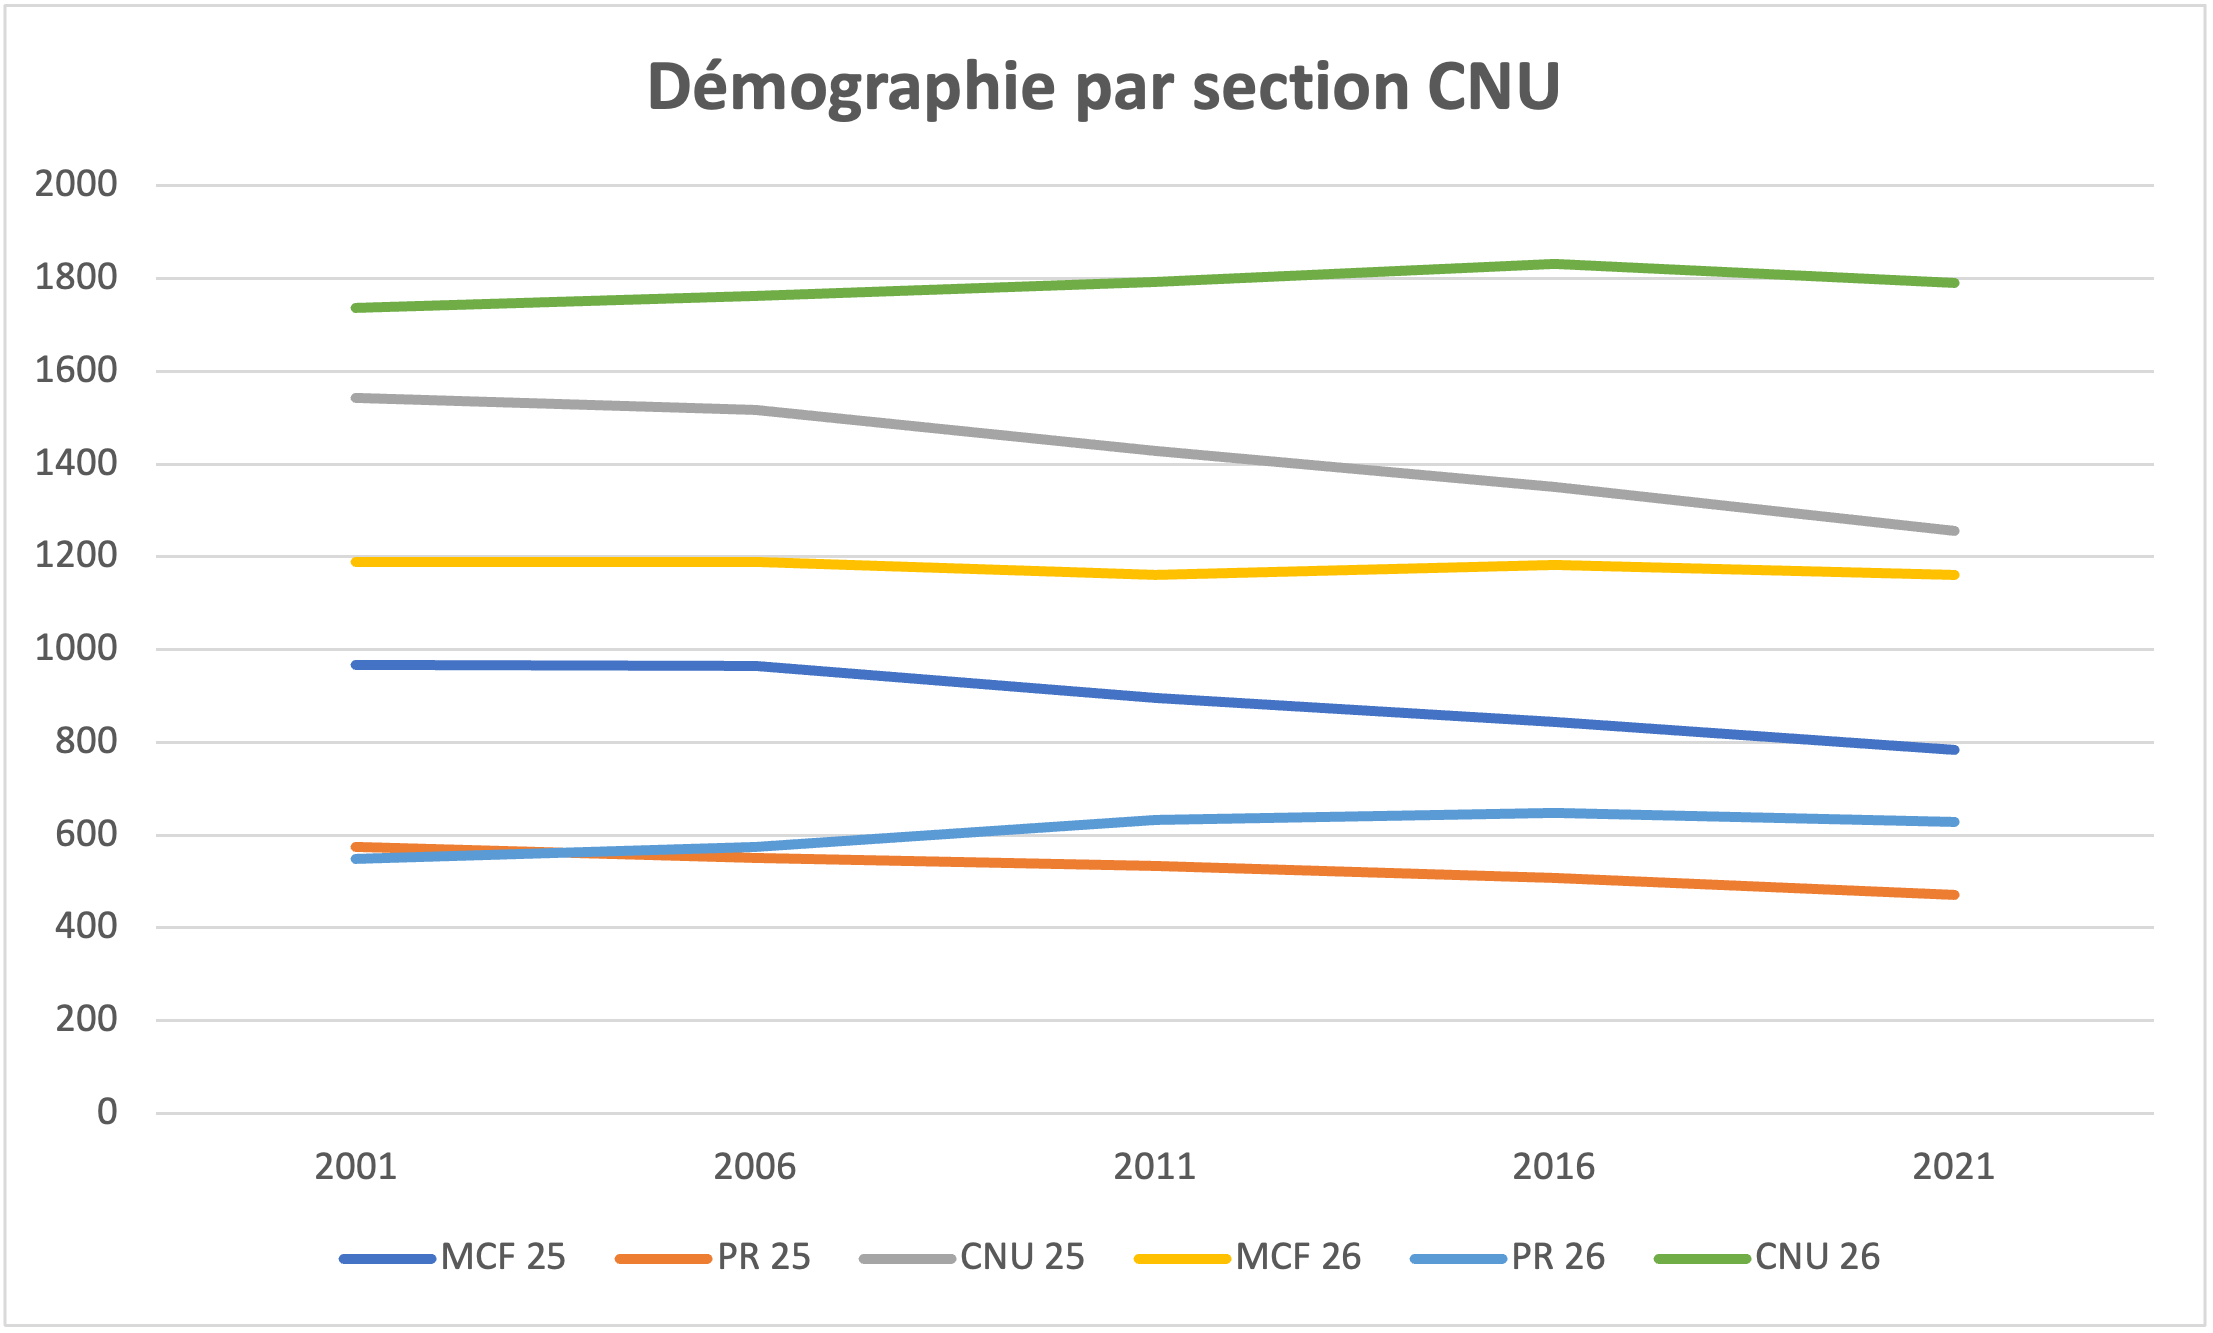
\includegraphics[width=8.5cm]{Images/cnu_demographie_2021}
}
\hfill
\subfloat[\'Evolution du nombre de postes publi\'es au concours pour les sections 25 et 26 du CNU (sessions synchronis\'ees)]{
\label{fig.cnu.postes}%
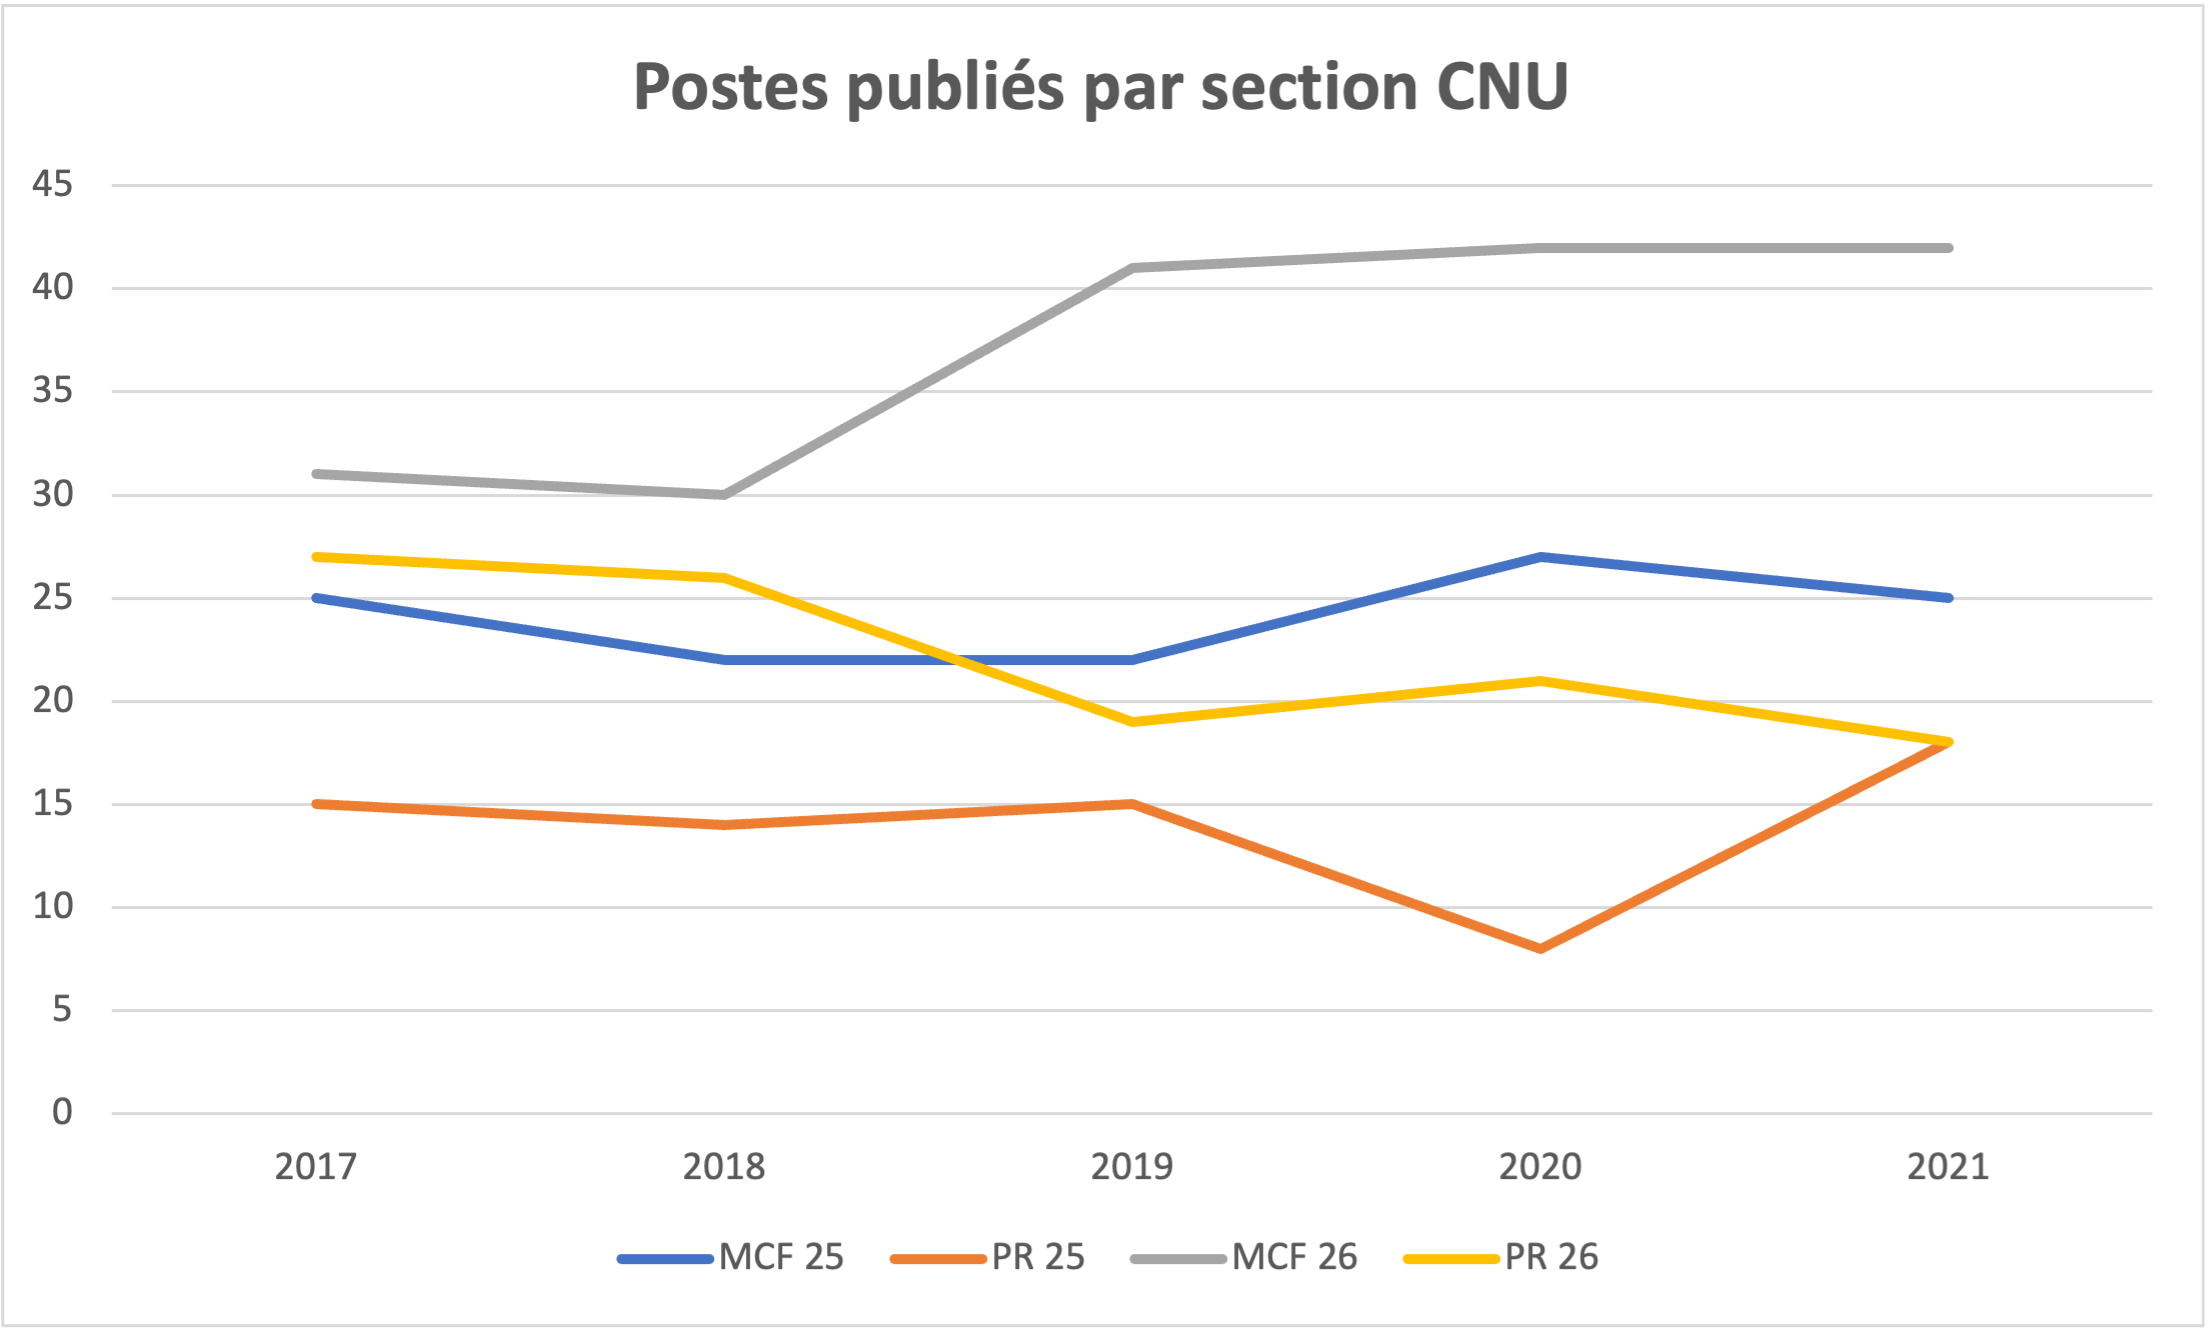
\includegraphics[width=8.5cm]{Images/cnu_nb_postes_2021}
}
\hfill
\begin{center}
\subfloat[\'Evolution du taux de pression (\textit{i.e.}, nombre de candidat\mp e\mp s/nombre de postes) pour les sections 25 et 26 du CNU (sessions synchronis\'ees)]{\label{fig.cnu.pression}%
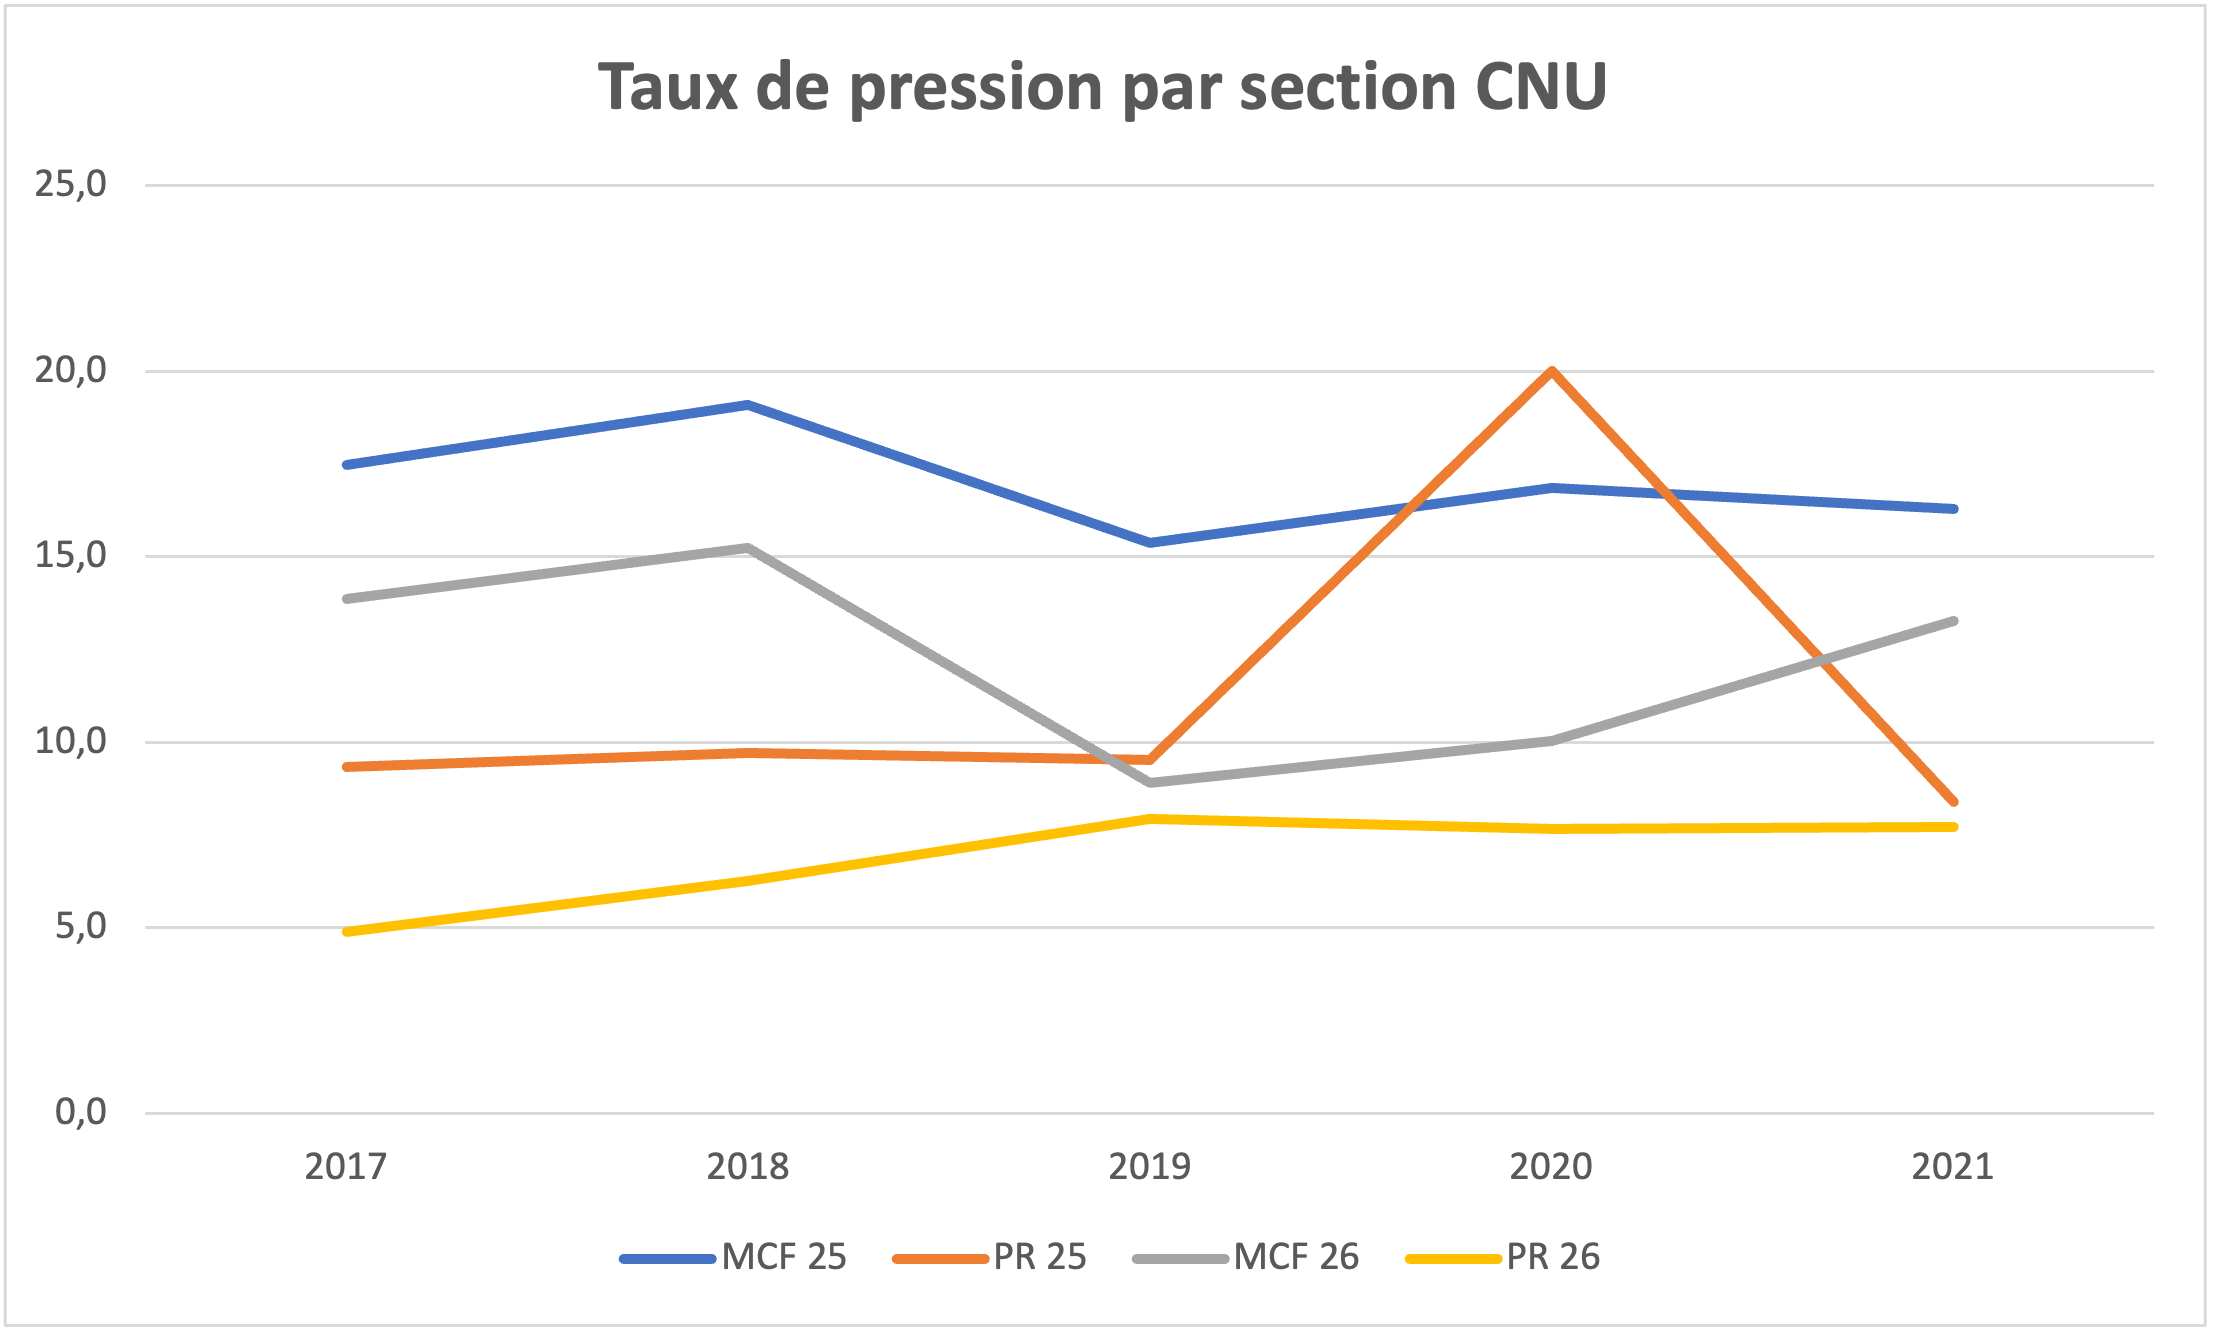
\includegraphics[width=8.5cm]{Images/cnu_taux_pression_2021}
}
\end{center}
\caption{Statistiques des postes d'enseignant\mp e\mp s-chercheur\mp euses au minist\`ere (MESRI)}
\label{fig.cnu}
\end{figure}


%\begin{figure}[p]
%\subfloat[\'Evolution du nombre de qualifi\'e\mp e\mp s]{\label{fig.qualif}%
%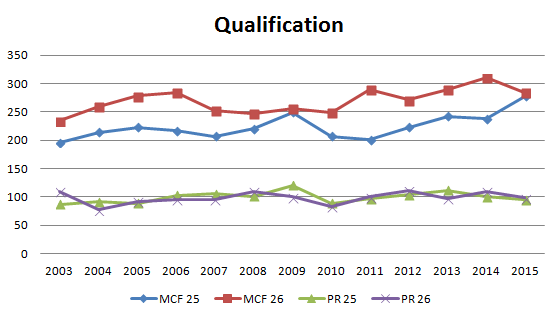
\includegraphics[width=8.5cm]{Images/qualif}
%}
%\hfill
%\subfloat[\'Evolution du nombre de postes]{\label{fig.postes}%
%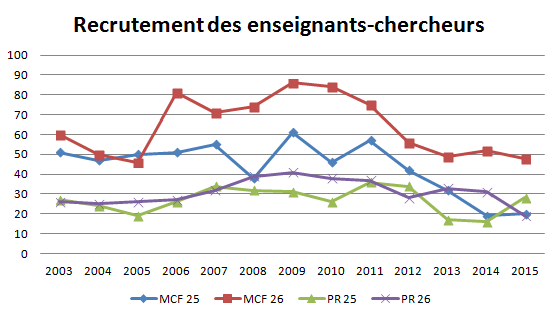
\includegraphics[width=8.5cm]{Images/recrut_EC}
%}
%\caption{Statistiques de recrutement en sections 25 et 26 du CNU (sessions synchronis\'ees)}\label{fig.recrut}
%\end{figure}

\paragraph*{Sources} Ces donn\'es ont \'et\'e compil\'ees \`a partir de rapports publics que nous vous invitons \`a consulter pour avoir davantage de d\'etails
\begin{itemize}
\item CNU : 
\url{https://www.enseignementsup-recherche.gouv.fr/fr/fiches-demographiques-des-sections-du-conseil-national-des-universites-cnu-83047}
\item Rapport sur la parit\'e dans la communaut\'e : \url{https://parite.math.cnrs.fr/effectifs.html}
\end{itemize}

% --- \`a mettre \`a jour
%Si l'on regarde plus en d\'etails les op\'erations de recrutement sur la d\'ecennie pass\'ee, on
%constate une d\'ecorr\'elation entre le nombre de qualifi\'e\mp e\mp s (constant voire en augmentation pour les MCF en section~26 
%-- voir Figure~\ref{fig.qualif})
%et le nombre de postes ouverts (voir Figure~\ref{fig.postes}). 
%Quant \`a l'\'ecart entre la date de qualification et la date de recrutement, il n'\'evolue pas de mani\`ere flagrante
%(voir Table~\ref{tab.recrut.anter}) : l'essentiel des recrutements s'effectue dans les 2 ans suivant la qualification.

%\begin{table}
%\begin{center}
%\begin{tabular}{*{7}{c}}
%\toprule
%&& $N-4$ & $N-3$ & $N-2$ & $N-1$ & $N$ \\
%\midrule
%2015 	& PR 25 & 1 & 3 & 5 & 6 & 7 \\
%	& PR 26 &  & 1 & 2 & 5 & 8 \\
%	& MCF 25 &  & 3 &  & 6 & 7 \\
%	& MCF 26 & 3 & 1 & 4 & 14 & 14 \\
%	\midrule
%2014 	& PR 25 &  &  & 2 & 2 & 7 \\
%	& PR 26 & 1 & 3 & 6 & 4 & 10 \\
%	& MCF 25 &  & 2 & 1 & 6 & 7 \\
%	& MCF 26 & 1 & 1 & 3 & 16 & 23 \\
%\midrule
%2013 	& PR 25 & 1 & 2 & 3 & 2 & 2 \\
%	& PR 26 & 1 & 1 & 1 & 5 & 15 \\
%	& MCF 25 &  & 3 & 1 & 9 & 17 \\
%	& MCF 26 &  &  & 5 & 13 & 25 \\
%\midrule
%2012	& PR 25 &  & 2 & 7 & 7 & 10 \\
%	& PR 26 & 2 & 2 & 2 & 5 & 10 \\
%	& MCF 25 & 1 & 5 & 1 & 12 & 21 \\
%	& MCF 26 & 1 & 1 & 6 & 13 & 32 \\
%\midrule
%2011 	& PR 25 & 1 & 3 & 2 & 5 & 15 \\
%	& PR 26 & 2 & 2 & 4 & 2 & 12 \\
%	& MCF 25 & 1 & 4 & 4 & 13 & 29 \\
%	& MCF 26 &  & 4 & 3 & 9 & 48 \\
%\midrule
%2010 	& PR 25 &  &  & 2 & 9 & 10 \\
%	& PR 26 &  & 1 & 3 & 7 & 14 \\
%	& MCF 25 &  & 3 & 6 & 9 & 22 \\
%	& MCF 26 &  & 6 & 9 & 13 & 43 \\
%\midrule
%2009	& PR 25 & 2 & 3 & 6 & 13 & 24 \\
%	& PR 26 & 3 & 2 & 4 & 17 & 26 \\
%	& MCF 25 &  & 3 & 12 & 18 & 21 \\
%	& MCF 26 &  & 3 & 8 & 12 & 44 \\
%\bottomrule
%\end{tabular}
%\caption{Temps \'ecoul\'e entre la qualification et le recrutement (ann\'ee $N$)}\label{tab.recrut.anter}
%\end{center}
%\end{table}
%
%


%%%%%%%%%%%%%%%%%%%%%%%%%%%%%%%%%%%%%%%%%%%%%
\section{Recrutement}
\label{recrutement}

Pour l'ensemble des disciplines, l'acc\`es aux corps
des ma\^itres de conf\'erences et des professeur\mp e\mp s des universit\'es comporte
g\'en\'eralement 2 \'etapes~:
\begin{enumerate}
\item la qualification aux fonctions
de ma\^\i tre de conf\'erences et/ou aux fonctions de professeur\mp e des
universit\'es;
\item les concours de recrutement ouverts dans chaque \'etablissement
d'enseignement sup\'erieur aux candidats et candidates pr\'ealablement
qualifi\'e\mp e\mp s.
\end{enumerate}

La qualification est une \'etape obligatoire pour \^etre \'eligible \`a une candidature \`a l'un de ces 2 corps. Pour les MCF titulaires et EC titulaires assimil\'e\mp e\mp s au corps des ma\^itres de conf\'erences relevant de la fonction publique française, la qualification est de droit apr\`es l'obtention de l'Habilitation \`a Diriger des Recherches (HDR). En cons\'equence, ils/elles ne doivent plus faire de demande de qualification aux fonctions de professeur\mp e des universit\'es. \`A l'exception de ce cas de figure, le processus de qualification est supervis\'e par le Conseil national des universit\'es (CNU : le fonctionnement de cet organisme est d\'ecrit en d\'etail dans le chapitre \ref{CNU}). 


La proc\'edure de recrutement proprement dite est quant \`a elle g\'er\'ee de mani\`ere autonome par les universit\'es elles-m\^emes. Pour chaque poste au concours, un jury, appel\'e comit\'e de s\'election, est constitu\'e ({\em cf.} Section \ref{sec. comiteselection}). Le comit\'e de s\'election examine les dossiers, \'etablit la liste des candidates et candidats qu'il souhaite entendre, et apr\`es avoir proc\'ed\'e aux auditions, il d\'elib\`ere sur les candidatures et \'emet un classement, \`a la majorit\'e des voix de ses membres. C'est au vu de l'avis \'emis par le comit\'e de s\'election que le Conseil d'administration propose le nom de la candidate ou du candidat s\'electionn\'e\mp e ou, le cas \'ech\'eant, une liste de candidat\mp e\mp s class\'e\mp e\mp s par ordre de pr\'ef\'erence.

Des informations sur les phases de qualification et de concours de recrutement peuvent \^etre trouv\'ee sur le site du minist\`ere (Galaxie) : \url{https://www.galaxie.enseignementsup-recherche.gouv.fr/ensup/candidats.html} ou sur le site de l'Op\'eration Postes \url{http://postes.smai.emath.fr}.



\subsection{Comit\'e de s\'election}\label{sec. comiteselection}
\index{Comit\'e de s\'election}

Les textes relatifs au comit\'e de s\'election peuvent \^etre trouv\'es au lien suivant :
\href{https://www.legifrance.gouv.fr/loda/id/JORFTEXT000000520453/2023-04-15/}{D\'ecret 84-431 du 6 juin 1984, version consolid\'ee du 01 janvier 2015}. 
On pourra aussi consulter le Code de l'Education, article L952-6-1 sur le
site \url{https://www.legifrance.gouv.fr/}.


Un comit\'e de s\'election est constitu\'e pour chaque emploi \`a pourvoir. Il constitue le jury du concours 
(D\'ecision du Conseil d'Etat 316927 du 15 d\'ecembre 2010 ; 317314 et 329584 du 9 f\'evrier 2011). 
Le Conseil d'administration, si\'egeant en formation
restreinte aux repr\'esentants \'elus des enseignant\mp e\mp s-chercheur\mp euse\mp s, des chercheur\mp euse\mp s et personnels assimil\'es, d\'elib\`ere
une premi\`ere fois pour pr\'eciser l'effectif total du comit\'e, entre 8 et 16 personnes, le nombre des membres choisis hors de
l'\'etablissement et le nombre de ceux choisis parmi les enseignants et enseignantes de la discipline concern\'ee. Au cours d'une
seconde d\'elib\'eration, il adopte la liste des membres, lesquels sont propos\'es par le\mp la pr\'esident\mp e ou le\mp la directeur\mp ice de
l'\'etablissement qui a recueilli l'avis de la Commission de la recherche.

Le comit\'e de s\'election est compos\'e de membres ext\'erieurs et de membres \og locaux\fg{}. Il si\`ege valablement si la moiti\'e de ses membres sont pr\'esents \`a la s\'eance, parmi lesquels une moiti\'e au moins de membres ext\'erieurs \`a l'\'etablissement. Sont consid\'er\'es comme membres ext\'erieurs \`a l'\'etablissement les enseignant\mp e\mp s-chercheur\mp euse\mp s et personnels assimil\'es qui ne sont pas \'electeur\mp ice\mp s pour les \'elections
au Conseil d'administration ; peuvent \^etre choisis des universitaires et des chercheuses et chercheurs d'institutions \'etrang\`eres,
d'un rang au moins \'egal \`a celui auquel postulent les candidat\mp e\mp s. La composition de chaque comit\'e est rendue
publique avant le d\'ebut de ses travaux.

Lorsqu'il s'agit d'un recrutement de ma\^itre de conf\'erences, le comit\'e de s\'election est compos\'e \`a parit\'e de MCF
et personnels assimil\'es et de PR et personnels assimil\'es. Pour un recrutement de professeur\mp e, seuls des PR et
personnels assimil\'es doivent former le comit\'e. Le Conseil d'administration choisit le ou la pr\'esident\mp e du comit\'e parmi les
membres du comit\'e.

Le comit\'e doit comprendre autant de femmes que d’hommes, avec des dispositions transitoires pour les comit\'es PR de certaines sections du CNU 
(comme la 25\`eme section) o\`u le pourcentage de femmes est faible.

Il faut signaler que nul ne peut appartenir simultan\'ement \`a des comit\'es de s\'election en activit\'e dans plus de 3
\'etablissements. Un comit\'e cesse son activit\'e \`a la date \`a laquelle il transmet ses avis au Conseil d'administration
de l'\'etablissement.

Un comit\'e de s\'election peut \^etre commun \`a plusieurs \'etablissements associ\'es \`a cette fin, notamment dans le
cadre d'un p\^ole de recherche et d'enseignement sup\'erieur ({\em cf.}, Section \ref{Regroupements}).

Le comit\'e de s\'election examine les dossiers des candidat\mp e\mp s \`a un recrutement, par la voie de la mutation, du
d\'etachement ou du concours. Notons que les articles 35 et 51 du statut \'etablissant la priorit\'e des mutations sur les concours ont \'et\'e abrog\'es : les mutations sont trait\'ees en m\^eme temps que les candidat\mp e\mp s demandant un premier recrutement en tant que MCF ou PR.
Le comit\'e de s\'election peut toutefois soumettre au Conseil d'administration des avis distincts pour chacune des 3 voies de recrutement.

Lors d'une seconde r\'eunion, le comit\'e de s\'election auditionne les candidat\mp e\mp s retenu\mp e\mp s, d\'elib\`ere sur les candidatures, \'emet un avis motiv\'e sur chaque candidature et, le cas \'ech\'eant, sur le classement retenu. Le comit\'e de s\'election se prononce \`a la majorit\'e des voix des membres pr\'esents. En cas de partage des voix, le pr\'esident du comit\'e a voix pr\'epond\'erante. Ces avis sont transmis au Conseil
d'administration, apr\`es quoi il est mis fin \`a l'activit\'e du comit\'e. Les avis sont communiqu\'es aux candidat\mp e\mp s sur leur demande. 

Le CA de l'\'etablissement si\`ege en formation
restreinte aux enseignant\mp e\mp s-chercheur\mp euse\mp s et personnels assimil\'es d'un rang au moins \'egal \`a celui de l'emploi
postul\'e. Il d\'elib\`ere \`a partir des avis formul\'es par le comit\'e de s\'election et peut, s'il l'estime n\'ecessaire, se faire communiquer toute pi\`ece du dossier des candidat\mp e\mp s. Il propose au ministre charg\'e de l'enseignement sup\'erieur le nom de la candidate ou du candidat s\'electionn\'e\mp e ou une liste de candidat\mp e\mp s class\'e\mp e\mp s par ordre de pr\'ef\'erence. La nomination dans le corps des MCF rel\`eve toujours de la comp\'etence du ministre, celle dans le corps des PR de la comp\'etence du ou de la Pr\'esident\mp e de la R\'epublique.

Le\mp La pr\'esident\mp e ou le\mp la directeur\mp ice de l'\'etablissement peut \'emettre un avis d\'efavorable motiv\'e sur le candidat retenu par
le CA ou sur l'un ou l'une des candidat\mp e\mp s class\'e\mp e\mp s ; en aucun cas, il\mp elle ne peut modifier l'ordre de la liste de classement.
Lorsque l'emploi \`a pourvoir est affect\'e \`a une \'ecole ou \`a un institut faisant partie d'une universit\'e, le\mp la pr\'esident\mp e ou
le\mp la directeur\mp ice de l'\'etablissement ne peut transmettre le nom du candidat ou de la candidate s\'electionn\'e\mp e ou la liste de classement si,
dans les 15 jours suivant la r\'eunion du Conseil d'administration, le\mp la directeur\mp ice de l'\'ecole ou de l'institut a \'emis un
avis d\'efavorable motiv\'e sur ce recrutement.

Concernant les mutations, sont admis \`a faire acte de candidature \`a la mutation sur un poste donn\'e les MCF qui, \`a la date de cl\^oture des inscriptions de ce poste (indiqu\'ee sur le site du minist\`ere), ont exerc\'e des fonctions d'enseignant\mp e-chercheur\mp euse en position d'activit\'e pendant au moins 3 ans dans l'\'etablissement o\`u ils\mp elles sont affect\'e\mp e\mp s, le stage \'etant pris en compte dans la d\'etermination de cette m\^eme p\'eriode. S'ils\mp elles ne justifient pas, \`a cette date, de 3 ans de fonctions d'enseignant\mp e-chercheur\mp euse en position d'activit\'e dans l'\'etablissement o\`u ils\mp elles sont affect\'e\mp e\mp s, les candidat\mp e\mp s ne peuvent d\'eposer une demande de mutation qu'avec l'accord de leur chef d'\'etablissement d'affectation, donn\'e apr\`es avis favorable du Conseil d'administration en formation restreinte aux enseignant\mp e\mp s-chercheur\mp euse\mp s et assimil\'es de rang au moins \'egal, ainsi que, le cas \'ech\'eant, de la ou du directeur\mp ice de l'institut ou de l'\'ecole faisant partie de l'universit\'e.

Les membres d'un comit\'e de s\'election peuvent participer aux r\'eunions en utilisant tout moyen de 
t\'el\'ecom\-munication permettant leur identification et leur participation effective : ils et elles sont alors r\'eput\'e\mp e\mp s pr\'esent\mp e\mp s pour
tous les calculs de quorum et de majorit\'e ; toutefois le comit\'e ne peut si\'eger valablement si le nombre des
membres physiquement pr\'esents est inf\'erieur \`a quatre.
Les candidates et candidats s\'electionn\'e\mp e\mp s pour l'audition peuvent demander \`a \^etre entendu\mp e\mp s par les m\^emes moyens de
t\'el\'ecommunication.

\textbf{Lien utile\hspace{.5em}}\url{https://www.galaxie.enseignementsup-recherche.gouv.fr/ensup/etab_FAQ_comites_selection.html}.

\subsection{Ma\^\i tres de conf\'erences}

Les ma\^itres de conf\'erences sont recrut\'e\mp e\mp s par concours ouverts par \'etablissement.

\subsubsection*{1\iere{} \'etape : inscription sur la liste nationale de qualification}

Cette inscripion est obligatoire pour pouvoir participer \`a la
deux\`eme \'etape du concours. Tout titulaire d'un doctorat ou d'un
dipl\^ome \'equivalent peut poser sa candidature. D'autres voies
d'acc\`es, moins courantes, sont n\'eanmoins possibles : justifier de
3 ann\'ees d'activit\'e professionnelle effective au cours des six
ann\'ees pr\'ec\'edentes \`a l'exclusion des activit\'es
d'enseignant\mp e ou de chercheur\mp euse, \^etre enseignant\mp e associ\'e\mp e \`a temps
plein, \^etre d\'etach\'e\mp e dans le corps des ma\^itres de
conf\'erences ou bien appartenir au corps de charg\'e\mp e de recherche
ou \`a un corps de chercheur\mp euse. Les conditions et la forme de la
demande d'inscription sur la liste de qualification sont
pr\'ecis\'ees dans un arr\^et\'e publi\'e chaque ann\'ee au Journal
officiel.

Habituellement, les candidatures se d\'eclarent entre mi-septembre et mi-octobre, 
par inscription sur le site \href{https://galaxie.enseignementsup-recherche.gouv.fr/antares/can/index.jsp}{Antares de Galaxie}.
Le nom des rapporteur\mp ice\mp s est mis en ligne \`a partir de la fin novembre et 
les candidats et candidates ont jusqu'\`a fin d\'ecembre pour envoyer leurs dossier apr\`es avoir au pr\'ealable soutenu
leur th\`ese (mi-d\'ecembre).
Le CNU se r\'eunit en d\'ebut d'ann\'ee et les listes des candidates et candidats qualifi\'e\mp e\mp s sont publi\'ees vers f\'evrier.

Le dossier de candidature comprend notamment une
description des activit\'es dans l'enseignement, la recherche ou
l'administration, et pr\'esente 3 exemplaires des travaux de la candidate ou du candidat,
ouvrages ou articles. Il est examin\'e par la section du CNU
comp\'etente pour la discipline. 

Pour tout renseignement sur la constitution du dossier et le calendrier exact de la proc\'edure de qualification, 
vous pouvez vous r\'ef\'erer \`a la page officielle sur Galaxie : \url{https://www.galaxie.enseignementsup-recherche.gouv.fr/ensup/cand_qualification_droit_commun.htm} ou au site de l'Operation Postes : \url{http://postes.smai.emath.fr/2015/CONCOURS/qualification/index.php}.

Le pourcentage de dossiers valid\'es
varie fortement suivant les disciplines. En math\'ematiques
(sections 25 et 26), il oscille autour de 75\,\% selon les bilans r\'edig\'es par les CNU 
\href{http://cnu25.emath.fr/}{25} et \href{http://cnu26.emath.fr/}{26} chaque ann\'ee. Notons que peut
\'eventuellement \^etre effectu\'ee
une demande d'inscription aupr\`es de plusieurs sections du CNU.

\subsubsection*{2\ieme{} \'etape~: les concours par \'etablissement}

Les concours sont ouverts dans les universit\'es, instituts ou
\'ecoles, en fonction du ou des postes \`a pourvoir. La plupart des
recrut\'e\mp e\mp s le sont sur le concours ouvert aux titulaires d'un
doctorat ou d'un dipl\^ome \'equivalent. Trois autres concours
existent n\'eanmoins. Le premier est r\'eserv\'e aux enseignantes et enseignants
titulaires du second degr\'e en fonction dans l'enseignement
sup\'erieur depuis 3 ans et titulaires d'un doctorat, et aux
pensionnaires ou anciens pensionnaires d'\'ecoles fran\c{c}aises \`a
l'\'etranger. Le deux\`eme est r\'eserv\'e aux candidats et candidates comptant
quatre ann\'ees d'activit\'e professionnelle effective au cours des
sept ann\'ees pr\'ec\'edentes, \`a l'exclusion des activit\'es
d'enseignant\mp e ou de chercheur\mp euse, et aux enseignant\mp e\mp s associ\'e\mp e\mp s \`a
temps plein.
Le dernier est r\'eserv\'e aux enseignant\mp e\mp s titulaires de l'Ecole nationale sup\'erieure d'arts et m\'etiers (ENSAM).

Les concours sont ouverts par arr\^et\'e du ministre charg\'e de
l'enseignement sup\'erieur. Les conditions et les modalit\'es du
d\'ep\^ot des candidatures sont pr\'ecis\'ees dans les arr\^et\'es
publi\'es au Journal officiel. Les candidatures sont
appr\'eci\'ees par les instances comp\'etentes des
\'etablissements~:
les comit\'es de s\'election et le Conseil d'administration.

L'\^age moyen du recrutement sur un poste de ma\^\i  tre de
conf\'erences \'etait en 2021 de 33 ans toutes sections sciences confondues. Pour obtenir d'autres statistiques, vous pouvez consulter les bilans des campagnes de recrutement mis en ligne r\'e\-gu\-li\`erement :
{\url{https://www.enseignementsup-recherche.gouv.fr/cid22708/bilans-statistiques.html}}

\subsection{Professeur\mp e\mp s des universit\'es}

Sous r\'eserve des dispositions particuli\`eres concernant les disciplines juridiques, politiques,
\'economiques et de gestion, les professeur\mp e\mp s des universit\'es sont recrut\'e\mp e\mp s par concours ouverts par \'etablissement.

\subsubsection*{1\iere{} \'etape : inscription sur la liste nationale de qualification}

Cette inscripion est obligatoire pour pouvoir participer \`a la deux\`eme \'etape du concours. N\'eanmoins, les MCF titulaires et EC titulaires assimil\'e\mp e\mp s au corps des ma\^itres de conf\'erences relevant de la fonction publique française n'ont d\'esormais plus de d\'emarches particuli\`eres \`a faire car ils sont r\'eput\'es qualifi\'es apr\`es l'obtention de l'Habilitation \`a Diriger des Recherches (HDR). Ne doivent donc faire la demande de qualification aux fonctions de professeur\mp e des universit\'es que les personnes titulaires de l'habilitation \`a diriger des recherches (HDR) ou d'un dipl\^ome \'equivalent n'ayant pas ce statut.

D'autres voies d'acc\`es, moins courantes, sont \'egalement possibles :
justifier de cinq ann\'ees d'activit\'e professionnelle effective au cours des huit ann\'ees pr\'ec\'edentes,
\`a l'exclusion des activit\'es d'enseignant\mp e ou de chercheur\mp euse,
\^etre enseignant\mp e associ\'e\mp e \`a temps plein,
\^etre d\'etach\'e\mp e dans le corps des professeur\mp e\mp s des universit\'es
ou bien appartenir au corps de directeur\mp ice\mp s de recherche ou \`a un corps de chercheur\mp euse.

Les statistiques de qualification sont de plus de 80\,\% dans les CNU 25 et 26.

\subsubsection*{2\ieme{} \'etape : les concours par \'etablissement}

Les concours sont ouverts dans les universit\'es, instituts ou \'ecoles, en fonction du ou des postes \`a pourvoir.
La plupart des recrut\'e\mp e\mp s le sont sur le concours ouvert aux titulaires d'une HDR ou d'un dipl\^ome \'equivalent.
Trois autres concours existent n\'eanmoins.

Le premier est r\'eserv\'e
aux MCF titulaires d'une HDR qui ont accompli cinq ann\'ees de service dans l'enseignement sup\'erieur ou qui ont \'et\'e charg\'e\mp e\mp s, 
depuis au moins 4 ans, d'une mission de coop\'eration culturelle,
scientifique et technique.

Le deux\`eme est r\'eserv\'e aux MCF titulaires de l'HDR qui ont accompli dix ann\'ees de service
(dont cinq en qualit\'e de MCF titulaire ou stagiaire) dans un \'etablissement d'enseignement sup\'erieur
de la Communaut\'e europ\'eenne, d'un \'etat faisant partie de l'accord sur l'espace \'economique
europ\'een,
ou dans un autre \'etablissement d'enseignement sup\'erieur au titre d'une mission de coop\'eration culturelle scientifique et technique, 
ou dans un \'etablissement public \`a caract\`ere scientifique et technologique.
Notons que la proc\'edure d'inscription sur la liste de qualification n'existe pas pour ce concours.
Le CNU formule, a posteriori, un avis sur les candidats retenus par l'\'etablissement.

Le dernier concours est ouvert
aux candidat\mp e\mp s ayant six ann\'ees d'activit\'e professionnelle effectives
durant les neuf ann\'ees pr\'ec\'edentes,
\`a l'exclusion des activit\'es d'enseignant\mp e ou de chercheur\mp euse,
aux enseignant\mp e\mp s associ\'e\mp e\mp s \`a temps plein,
aux MCF membres de l'Institut universitaire de France
et \`a des directeur\mp ice\mp s de recherche qui ont effectu\'e une d\'emarche de mobilit\'e
vers l'enseignement sup\'erieur, pour des nominations comme professeur\mp e des universit\'es de premi\`ere classe.

L'\^age moyen du recrutement sur un poste de  professeur\mp e des
universit\'es \'etait en 2021 de 45 ans toutes sections sciences confondues. Pour obtenir d'autres statistiques, vous pouvez consulter les bilans des campagnes de recrutement mis en ligne r\'e\-gu\-li\`erement :
{\url{https://www.enseignementsup-recherche.gouv.fr/cid22708/bilans-statistiques.html}}

%%%%%%%%%%%%%%%%%%%%%%%%%%%%%%%%%%%%%%%%%%%%%%%
\section{L'affectation}

Tout\mp e enseignant\mp e-chercheur\mp euse est rattach\'e\mp e \`a une unit\'e de formation
et de recherche (UFR), un d\'epar\-te\-ment, ou \`a un organe
\'equivalent, suivant l'\'etablissement d'affectation.

En ce qui concerne la recherche, il existe plusieurs types de
laboratoires de recherche dont les principaux, en ce qui concerne
les math\'ematiques, sont~:
\begin{itemize}
	\item les unit\'es mixtes de recherche (UMR)~: ces laboratoires,
		localis\'es dans les universit\'es, sont rattach\'es au CNRS~;
	\item les \'equipes d'accueil (EA)~: ces laboratoires sont
		reconnus et habilit\'es par le minist\`ere seul.
\end{itemize}

Dans certains \'etablissements, tels que 
les \'ecoles sup\'erieures du professorat et de l'\'education (ESPE), ancien IUFM,
ou encore dans
certaines \'ecoles d'ing\'enieurs ou IUT, il n'y a pas assez
d'enseignant\mp e\mp s-chercheur\mp euse\mp s par discipline pour monter une \'equipe de
recherche.
\index{Ecoles sup\'erieures du professorat et de l'\'education (ESPE)}
Quel que soit l'endroit de votre affectation, n'h\'esitez pas
\`a contacter le responsable du laboratoire de math\'e\-matiques le plus
proche pour demander votre rattachement. Cette demande sera, dans la
plupart des cas, re\c cue tr\`es positivement et vous permettra de ne
pas rester scientifiquement isol\'e\mp e. Tout\mp e enseignant\mp e-chercheur\mp euse
devrait \^etre rattach\'e\mp e \`a une \'equipe de
recherche ! Pour trouver les coordonn\'ees de ces structures, n'h\'esitez pas \`a
consulter l'annuaire de la communaut\'e math\'e\-matique
fran\c caise. \url{https://annuaire.emath.fr}

Nous rappelons de plus que tout\mp e nouvel\mp le enseignant\mp e-chercheur\mp euse (comme tout nouveau fonctionnaire)
a le droit de pr\'esenter une demande de reconstitution de carri\`ere : elle permet de faire reconna\^\i tre tout emploi comportant une activit\'e de recherche pr\'ec\'edant l'embauche \`a fin d'avancement d'\'echelon \`a l'anciennet\'e.

%%%%%%%%%%%%%%%%%%%%%%%%%%%%%%%%%%%%%%%%%%%%%%%
\section{L'\'evaluation}

Les EC sont \'evalu\'e\mp e\mp s lors de quelques moments importants de leurs carri\`eres.
Cette \'evaluation est (presque) exclusivement bas\'ee sur ses activit\'es de recherche
et d'encadrement doctoral (dans une moindre mesure).
Elle intervient lors~:
\begin{itemize}
\item de sa titularisation, au bout d'un an, sur d\'ecision de la Commission de la recherche de l'\'etablissement~;
\item des demandes de promotion, de primes (dispositif RIPEC),
de cong\'es pour recherche ou conversion
th\'ematique (CRCT), de d\'el\'egation et de d\'etachement (dans les
3 derniers cas, l'\'evaluation se fait surtout sur le projet de
recherche)~;
\item du passage de l'habilitation \`a diriger des recherches (HDR)~;
\item des concours de recrutement.
\end{itemize}
Un\mp e EC est \'egalement \'evalu\'e\mp e lors de l'\'evaluation de son laboratoire
et de son \'etablissement,
\'evaluations collectives par le Haut Conseil de l'Evaluation de la
Recherche et de l'Enseignement Sup\'erieur (HCERES, {\em cf.}, Chapitre \ref{HCERES}).
Les activit\'es de recherche de tous les membres du
laboratoire sont alors prises en compte, et la notion de \og publiant\fg{} est
alors utilis\'ee.
%
%Rappelons que le fonctionnement de l'HCERES est d\'etaill\'e dans le chapitre \ref{HCERES},
%et que de nombreuses informations sont disponibles sur son site
%\url{www.hceres.fr/}

D'autre part, le d\'ecret 2009-461 du 29 avril 2009 introduisait dans les missions du CNU l'\'evaluation individuelle des EC. 
Ce d\'ecret a \'et\'e fortement rejet\'e par tou\mp te\mp s les acteur\mp ice\mp s de la communaut\'e, en particulier les CNU 25 et 26.
Un moratoire avait alors \'et\'e annonc\'e pour la session 2012--2013. 
Ce d\'ecret a \'et\'e remplac\'e depuis par le d\'ecret 2014-997 du 2 septembre 2014 qui pr\'econise
d\'esormais un \og suivi de carri\`ere\fg{} quiquennal rempla\c{c}ant l'\'evaluation individuelle. Le suivi de carri\`ere est obligatoire mais certaines sections dont les sections 25 et 26 ont refus\'e de le faire. Parmi les m\'edias de contestation, citons par exemple : \url{http://www.sauvonsluniversite.com/spip.php?article3423}.

% \textit{Motions \'evaluation adopt\'ees le 2 f\'evrier 2010 par la section 25 (Math\'ematiques appliqu\'ees et applications des math\'ematiques) du CNU}
% 
% Motion 1 : Les membres de la section 25 du CNU r\'eunis le 2 f\'evrier 2010 rappellent que durant le mandat en cours ils refuseront de si\'eger pour une \'eventuelle session d'\'evaluation quadriennale.
% 
% \textit{Motions \'evaluation adopt\'ees le 3 f\'evrier 2010 par la section 26 (Math\'ematiques appliqu\'ees et applications des math\'ematiques) du CNU}
% 
% La section 26 du CNU a pris position le 4 f\'evrier 2010 contre la proposition de la CP-CNU de donner un avis sur tous les dossiers de demande de promotions, m\^eme pour les candidats \`a qui ne sera pas accord\'ee de promotion. La section consid\`ere en effet que c'est inutile, voire n\'efaste, car cela revient \`a mettre le doigt dans l'engrenage de l'\'evaluation quadriennale. Voici les motions vot\'ees :
% 
% Point 1 : \og Lors de la session d'attribution des promotions, la section CNU 26 n'\'emettra pas d'avis sur les dossiers des coll\`egues non promus." - Adopt\'e \`a l'unanimit\'e
% 
% Point 2 : \og Les membres de la section 26 r\'eunis le 3 f\'evrier 2010 rappellent leur refus de si\'eger pour une \'eventuelle session d'\'evaluation quadriennale durant leur mandat." - Unanimit\'e moins une abstention.


\index{Evaluation ! \`a l'universit\'e}
\index{Publiants}
\index{Haut Conseil de l'Evaluation de la
Recherche et de l'Enseignement Sup\'erieur (HCERES)}
\index{Cong\'e pour recherche ou conversion th\'e\-ma\-ti\-que (CRCT)}
\index{Habilitation \`a diriger des recherches (HDR)}

%%%%%%%%%%%%%%%%%%%%%%%%%%%%%%%%%%%%%%%%%
\section{L'enseignement}
\label{enseignement}

Outre leurs activit\'es de recherche, les EC assurent des enseignements. Le service statutaire est de 192 heures \og \'equivalent TD\fg{}. 
La conversion est : 1h cours (en pr\'esentiel)= 1,5 h \'eq. TD, les TP \'etant compt\'es comme les TD sauf s'il sont effectu\'es en heures compl\'ementaires. Donc un EC peut faire par exemple 192h de TD ou 60h de cours et 102h de TD 
({\em cf.}, \href{http://www.legifrance.gouv.fr/affichTexte.do?cidTexte=JORFTEXT000020552216&dateTexte=&categorieLien=id}{D\'ecret num\'ero 2009-460 du 23 avril 2009}).


\`A ce service commun, peuvent s'ajouter des heures
compl\'ementaires, parfois en nombre limit\'e dans certains \'etablissements (\href{http://www.legifrance.gouv.fr/affichTexte.do?cidTexte=JORFTEXT000000315917&dateTexte=20121122}{voir la modification de l'Arr\^et\'e du 6 novembre 1989 fixant les taux de r\'emun\'eration des heures compl\'ementaires}). Une heure est r\'emun\'er\'ee par une indemnit\'e non soumise \`a retenue pour pension et fix\'ee \`a 61,35 \euro~ pour les cours, 40,91 \euro~ pour les travaux pratiques et 27,26 \euro~ pour les travaux pratiques.

%\begin{table}[!ht]
%\begin{center}
%\begin{tabular}{|c|c|c|}
%\hline
%Cours & Travaux dirig\'es & Travaux pratiques\\
%\hline
%61,35 \euro & 40,91 \euro & 27,26 \euro\\
%\hline
%\end{tabular}
%\end{center}
%\end{table}

Les enseignant\mp e\mp s b\'en\'eficiant d'une d\'echarge statutaire de service de quelque
nature qu'elle soit, les enseignant\mp e\mp s en cong\'e pour recherche ou
conversion th\'ematique (CRCT), en cong\'e parental ou b\'en\'eficiant d'une
d\'echarge sollicit\'ee ne peuvent effectuer d'heures
compl\'ementaires. Notons enfin
que, ni les PRAG b\'en\'eficiant d'une d\'echarge pour
pr\'eparer leur th\`ese ou faire de la recherche,
ni les contrats doctoraux charg\'es d'enseignement,
ni les ATER ne peuvent effectuer d'heures compl\'ementaires.

La loi LRU sp\'ecifie express\'ement que le Conseil
d'administration pourra d\'efinir les principes g\'en\'eraux de
r\'epartition des obligations de service des personnels enseignants
entre leurs diff\'erentes activit\'es (enseignement, recherche,
administration, valorisation...), dans le respect des dispositions
statutaires et en fonction des besoins de l'\'etablissement.

\index{R\'ef\'erentiel des t\^aches}
\label{referentiel}
L'arr\^et\'e du 31 juillet 2009 institue \`a cet effet un r\'ef\'erentiel
national d'\'equivalence horaire, dont doit se saisir chaque \'etablissement
pour fixer son r\'ef\'erentiel propre. Ce travail est encore en cours dans bon nombre
d'\'etablissements, qui ont aussi le loisir, par l'interm\'ediaire de son pr\'esident,
de moduler le service d'un ou d'une enseignant\mp e-chercheur\mp euse \`a la hausse ou \`a la baisse (avec l'accord
explicite de l'int\'eress\'e). Pour plus de renseignements, on peut lire l'article 7 du d\'ecret 84-431 sur
\url{https://www.legifrance.gouv.fr/}.

\index{Travaux dirig\'es (TD)}\index{Travaux pratiques (TP)}
\index{R\'ef\'erentiel horaire}

%%%%%%%%%%%%%%%%%%%%%%%%%%%%%%%%%%%%%%%%%
\section{Carri\`ere et r\'emun\'eration}
\label{salairesEC}

Comme pour tout fonctionnaire, le traitement d'un\mp e EC est constitu\'ee
d'une r\'emun\'eration principale \`a laquelle s'ajoutent des indemnit\'es et des primes.

La r\'emun\'eration principale d'un\mp e EC augmente
p\'e\-rio\-di\-quement au fur et \`a mesure qu'il gravit les
\'echelons \`a l'int\'erieur de son grade. Cette progression se fait \`a l'anciennet\'e ({\em cf.}, Tables \ref{tab.avanc.MCF} et \ref{tab.avanc.PR}).
A chaque \'echelon correspond en effet un indice qui d\'etermine le montant de la
r\'emun\'eration principale. L'indice de r\'emun\'eration auquel le\mp la candidat\mp e est recrut\'e\mp e est d\'etermin\'e en fonction de ses dipl\^omes et de ses activit\'es professionnelles ant\'erieures. Le calcul est simple~: un point
d'indice a une certaine valeur fiduciaire (au 1er janvier 2023, la valeur est fix\'ee \`a 4,85 \euro) et le traitement est
calcul\'e par simple multiplication du nombre de points d'indice par
cette valeur nominale. La valeur du point d'indice est
r\'e\'evalu\'ee de mani\`ere \'episodique.
% \`A titre d'exemple, la valeur
% annuelle du point d'indice en date du 1er f\'evrier 2015 \'etait de
% 55,5635\,\euro{} brut. La pr\'ec\'edente r\'e\'evalutation, en
% date du 1er juillet 2010, correspond \`a une hausse de 0,5\,\% (ce qui,
% pour un MCF d\'ebutant, correspond \`a une augmentation de 10 euros
% brut mensuel). Notons que les r\'e\'evaluations successives depuis le 1er d\'ecembre
% 2002 correspondent \`a une augmentation totale de 5,85\, \%, et que l'inflation sur la m\^eme
% dur\'ee est d'environ 20,9\,\% d'apr\`es l'INSEE.

S'ajoutent ensuite \`a cette r\'emun\'eration principale diverses indemnit\'es
(r\'esidence, suppl\'ement familial)
et/ou diff\'erentes primes (RIPEC, primes administratives, ...)
ainsi que le paiement des \'eventuelles heures compl\'emen\-taires effectu\'ees
({\em cf.}, Section \ref{enseignement}).


\subsection{Grilles d'avancement et de salaires}\label{sec. grilles}

Le corps des MCF comporte 2 classes
(\textit{grades}):
\begin{itemize}
\item une classe normale, qui comprend 9 \'echelons~;
\item une hors-classe, qui comprend 6 \'echelons.
\end{itemize}

\begin{center}
\begin{table}[b!]
\begin{center}
\subfloat[MCF classe normale]{
\begin{tabular}{lcc}
\toprule
& Indice (INM)& Dur\'ee \\
\midrule
1\ier{} \'echelon &474&1 an \\
2\ieme{} \'echelon &531&2 ans et 10 mois\\
3\ieme{} \'echelon &584&2 ans et 10 mois\\
4\ieme{} \'echelon &643&2 ans et 10 mois\\
5\ieme{} \'echelon &693&2 ans et 10 mois\\
6\ieme{} \'echelon &739&3 ans et 6 mois\\
7\ieme{} \'echelon &769&2 ans et 10 mois\\
8\ieme{} \'echelon &803&2 ans et 10 mois\\
9\ieme{} \'echelon &830&\\
\bottomrule
\end{tabular}
}
\hfill
\subfloat[MCF hors-classe]{
\begin{tabular}{lcc}
\toprule
& Indice (INM)& Dur\'ee\\
\midrule
1\ier{} \'echelon &678&1 an\\
2\ieme{} \'echelon &716&1 an\\
3\ieme{} \'echelon &754&1 an\\
4\ieme{} \'echelon &796&1 an\\
5\ieme{} \'echelon &830&5 ans\\
6\ieme{} \'echelon & & \\
~\hspace{1cm}1\ier{} chevron &890&1 an\\
~\hspace{1cm}2\ieme{} chevron &925&1 an\\
~\hspace{1cm}3\ieme{} chevron &972& avancement \\
\'Echelon exceptionnel & & \\
~\hspace{1cm}1\ier{} chevron &972&1 an\\
~\hspace{1cm}2\ieme{} chevron &1013&1 an\\
~\hspace{1cm}3\ieme{} chevron &1067&  \\
\bottomrule
\end{tabular}
}
\caption{Grilles d'avancement des MCF}\label{tab.avanc.MCF}
\end{center}
\end{table}
\end{center}

\index{Ma\^\i tre de conf\'erences (MCF)!classe normale}
\index{Ma\^\i tre de conf\'erences (MCF)!hors-classe}

%\newpage
Le corps des PR comporte 3
classes (\textit{grades}):
\begin{itemize}
\item une seconde classe qui comprend 6 \'echelons~;
\item une premi\`ere classe qui comprend 3 \'echelons~;
\item une classe exceptionnelle qui comprend 2 \'echelons.
\end{itemize}

\begin{center}
\begin{table}[t!]
\begin{center}
\subfloat[PR seconde classe]{\small
\begin{tabular}{lcc}
\toprule
& Indice (INM)& Dur\'ee\\
\midrule
1\ier{} \'echelon &667&1 an\\
2\ieme{} \'echelon &705&1 an\\
3\ieme{} \'echelon &743&1 an\\
4\ieme{} \'echelon &785&1 an\\
5\ieme{} \'echelon &830&3 ans et 6 mois\\
6\ieme{} \'echelon & & \\
~\hspace{1cm}1\ier{} chevron &890&1 an\\
~\hspace{1cm}2\ieme{} chevron &925&1 an\\
~\hspace{1cm}3\ieme{} chevron &972& 3 ans et 6 mois\\
7\ieme{} \'echelon & &\\ 
~\hspace{1cm}1\ier{} chevron &972&1 an\\
~\hspace{1cm}2\ieme{} chevron &1013&1 an\\
~\hspace{1cm}3\ieme{} chevron &1067& \\
\bottomrule
\end{tabular}
}
\hfill
\subfloat[PR premi\`ere classe]{
\begin{tabular}{lcc}
\toprule
& Indice (INM)& dur\'ee\\
\midrule
1\ier{} \'echelon &830&3 ans\\
2\ieme{} \'echelon & &  \\
~\hspace{1cm}1\ier{} chevron &972&1 an\\
~\hspace{1cm}2\ieme{} chevron &1013&1 an\\
~\hspace{1cm}3\ieme{} chevron &1067&2 ans et 4 mois \\
3\ieme{} \'echelon & &  \\
~\hspace{1cm}1\ier{} chevron &1124&1 an\\
~\hspace{1cm}2\ieme{} chevron &1148&1 an\\
~\hspace{1cm}3\ieme{} chevron &1173& \\
\bottomrule
\end{tabular}
}

\subfloat[PR classe exceptionnelle]{
\begin{tabular}{lcc}
\toprule
& Indice (INM)& dur\'ee\\
\midrule
1\ier{} \'echelon & &  \\
~\hspace{1cm}1\ier{} chevron &1173&1 an\\
~\hspace{1cm}2\ieme{} chevron &1226&1 an\\
~\hspace{1cm}3\ieme{} chevron &1279& \\
2\ieme{} \'echelon & &  \\
~\hspace{1cm}1\ier{} chevron &1279&1 an\\
~\hspace{1cm}2\ieme{} chevron &1329&\\
\bottomrule
\end{tabular}
\normalsize}
\caption{Grilles d'avancement des PR}\label{tab.avanc.PR}
\end{center}
\end{table}
\end{center}


\index{Professeur\mp e des universit\'es (PR)!seconde classe}
\index{Professeur\mp e des universit\'es (PR)!premi\`ere classe}
\index{Professeur\mp e des universit\'es (PR)!classe exceptionnelle}


\`A l'exception des PR de classe exceptionnelle,
le passage d'un \'echelon au suivant (dans chaque classe) se fait
automatiquement, \`a l'{\em anciennet\'e}, selon le tempo indiqu\'e
dans les tableaux \ref{tab.avanc.MCF} et \ref{tab.avanc.PR}, o\`u l'on rapporte aussi les indices
nouveaux major\'es (INM). Pour le passage \`a la classe exceptionnelle, le nombre de promotions est calcul\'e chaque ann\'ee et d\'efini globalement, pour l'ensemble des sections, sous forme d'un pourcentage de promotions par rapport au nombre de \og promouvables\fg{} 
%({\em cf.}, par exemple le\href{www.legifrance.gouv.fr/affichTexte.do?cidTexte=JORFTEXT000025756970\&dateTexte=\&categorieLien=id}{lien sur Legifrance}.

Pour un\mp e MCF, le passage \`a la hors-classe se fait au {\em choix} (16 ans minimum
apr\`es le d\'ebut de carri\`ere~: il faut avoir atteint le
7\ieme{} \'echelon de la classe normale).
Pour un\mp e PR, le passage d'une classe \`a l'autre se fait \'egalement au {\em choix}.
Nous renvoyons \`a la section sur le Conseil national des universit\'es (CNU) pour la
description de l'attribution des promotions (\textit{c.f.}, Chapitre \ref{CNU}).

Des bonifications d'anciennet\'e peuvent \^etre accord\'ees aux EC
qui ont assur\'e un mandat de pr\'esident\mp e
ou de directeur\mp ice d'\'etablissement public d'enseignement sup\'erieur
ou qui s'engagent dans une d\'emarche de
mobilit\'e (par exemple une bonification d'anciennet\'e d'un an
pour un s\'ejour d'un an dans un organisme d'enseignement sup\'erieur
ou de recherche d'un autre \'etat de la Communaut\'e europ\'eenne,
{\em cf.}, le d\'ecret 2002-295 du 28 f\'evrier 2002).

\index{Conseil national des universit\'es (CNU)}
\index{Ma\^\i tre de conf\'erences (MCF)!promotions}
\index{Professeur des universit\'es (PR)!promotions}

On peut noter au passage que, d'apr\`es les donn\'ees de l'INSEE, le salaire initial d'un ou d'une ma\^\i tre de
conf\'erences (indice 454) a subi une diminution constante et r\'eguli\`ere
par rapport au SMIC de plus de 30\,\% depuis 1990 (passage de 2,07 au 01/01/1990 \`a 1,34 fois le SMIC au 01/01/2023)\ldots

%\subsection{Les indemnit\'es et les primes}

\subsection{Indemnit\'es et primes -- Le dispositif RIPEC}

La politique indemnitaire pour les EC est d\'efinie par la loi n° 2020-1674 du 24 d\'ecembre 2020 de programmation de la recherche pour les ann\'ees 2021 \`a 2030 (LPR). Les EC sont \'eligibles \`a des indemnit\'es statutaires et \`a des primes fix\'ees par le d\'ecret n° 2021-1895 du 29 d\'ecembre 2021 ayant conduit \`a la cr\'eation du r\'egime indemnitaire des personnels enseignants et chercheurs (RIPEC). Ce dispositif comprends 3 composantes. 

\textbf{Lien utile\hspace{.5em}}\url{https://www.enseignementsup-recherche.gouv.fr/fr/bo/22/Hebdo10/ESRH2204566X.htm}.

\subsubsection{La composante statutaire (C1)}
\label{ripec-C1}

Cette part indemnitaire est vers\'ee mensuellement \`a tous les EC qui accomplissent l'int\'egralit\'e de leur service. Elle remplace depuis 2022 la prime de recherche et d'enseignement sup\'erieur (PRES) qui \'etait attribu\'ee aux enseignants-chercheurs (d\'ecret n° 89-775 du 23 octobre 1989). D'ici \`a 2030, le montant annuel de l'indemnit\'e sera fix\'e chaque ann\'ee par arr\^et\'e. En 2022, il \'etait de 2800 \euro.

Les personnels plac\'es en d\'el\'egation, en cong\'e pour recherches ou conversions th\'ematiques ou en cong\'e pour projet p\'edagogique et aux personnels qui b\'en\'eficient de d\'echarges de service peuvent \'egalement b\'en\'eficier de cette ind\'emnit\'e. Ce n'est en revanche pas le cas des personnels qui perçoivent des r\'emun\'erations compl\'ementaires au titre de l'exercice d'une profession lib\'erale.

%Une prime annuelle de recherche est vers\'ee \`a toutes et tous les
%enseignant\mp e\mp s-chercheur\mp euse\mp s. Son montant est aujourd'hui de
%1244,98\,\euro{} brut. Elle est vers\'ee en 2 fois, aux mois de
%d\'ecembre et juillet. Elle est compatible avec le fait d'effectuer
%des heures compl\'ementaires, mais pas avec un cumul d'emploi.
%

\subsubsection{La composante fonctionnelle (C2)}

Cette indemnit\'e est li\'ee \`a l'exercices de fonctions ou responsabilit\'es particuli\`eres fix\'ees par le\mp la chef\mp fe de l'\'etablissement. Elle est vers\'ee mensuellement. Son montant annuel est plafonn\'e par arr\^et\'e minist\'eriel par groupes de fonctions ou de niveaux de responsabilit\'e. 

Tout comme la composante C1, il est n\'ecessaire de satisfaire ses obligations de service pour pouvoir en b\'en\'eficier. En revanche, \`a l'inverse de la composante C1, elle ne peut \^etre per\c{c}ues par les EC position de d\'el\'egation, en cong\'e pour recherches ou conversions th\'ematiques ou en cong\'e pour projet p\'edagogique, ou percevant des r\'emun\'erations compl\'ementaires au titre de l'exercice d'une profession lib\'erale.

\subsubsection{La prime individuelle (C3)}
\label{ripec-C3}

Cette prime remplace depuis 2022 la prime d'encadrement doctoral et de recherche (PEDR, d\'ecret n° 2009-851 du 8 juillet 2009). L'attribution de cette prime se fait suite un processus d'\'evaluation en plusieurs \'etapes.

Tout d'abord, les EC souhaitant b\'en\'eficier de cette prime doivent d\'eposer un dossier, comprenant notamment un rapport d'activit\'e de recherche et d'enseignement portant sur les 4 ann\'ees pr\'ec\'edant la candidature, sur l'application \href{https://www.galaxie.enseignementsup-recherche.gouv.fr/ensup/cand_RIPEC.htm}{ELARA de Galaxie}. Le CNU rend ensuite un avis unique (tr\`es favorable, favorable ou r\'eserv\'e) et pr\'ecise au titre de quelle mission (recherche, p\'edagogie, vie collective) la prime est propos\'ee. Il peut s'agir d'une de ces missions, de plusieurs ou de l'ensemble d'entre elles.

Une fois les dossiers \'evalu\'es par le CNU, ils sont transmis au conseil acad\'emique si\'egeant en formation restreinte aux EC et personnels assimil\'es (CAFR), ou \`a l'organe comp\'etent, de l'\'etablissement de rattachement de l'EC. Ce dernier d\'esigne 2 rapporteurs par candidat\mp e de rang au moins \'egal \`a celui du ou de la candidat\mp e. Sur la bases de ces 2 rapports, le CA rend \`a son tour un avis unique (tr\`es favorable, favorable ou r\'eserv\'e) sur l’ensemble du dossier du candidat, en pr\'ecisant \'egalement au titre de quelle mission (recherche, p\'edagogie ou vie collective), la prime est propos\'ee.  

Les 2 avis consultatifs du CNU et du CA sont ajout\'es au dossier, alors transmis au pr\'esident\mp e ou directeur\mp ice de l'\'etablissement de rattachement de l'EC qui arr\^ete les d\'ecisions d’attribution individuelle de la prime comprenant le montant, la ou les missions au titre de laquelle ou desquelles la prime sera attribu\'ee.  

La prime est attribu\'ee pour une dur\'ee de 3 ans et est vers\'ee mensuellement avec effet au 1er octobre de l'ann\'ee au titre de laquelle elle est attribu\'ee. Elle ne peut être cumul\'ee avec une autre prime individuelle. Tout comme la PEDR, les montants de cette primes sont variables et d\'ecid\'es localement en respectant une fourchette impos\'ee par le minist\`ere. En 2022, le montant annuel plancher est fix\'e \`a 3 500 \euro et le montant annuel maximum est fix\'e \`a 12 000 \euro. Les d\'ecisions des \'etablissements sont tr\`es diff\'erentes, certains utilisent un syt\`eme \`a plusieurs niveaux (par exemple distinction en fonction du rang ou de la mission) et d'autres fonctionnent sur un principe d'\'equit\'e entre tou\mp te\mp s pour en distribuer un plus grand nombre...

\`A noter que les enseignant\mp e\mp s-chercheur\mp euse\mp s plac\'e\mp e\mp s en d\'el\'egation aupr\`es de l'IUF b\'en\'eficie de droit de la prime individuelle. La demande s'effectue directement aupr\`es de l'\'etablissement. Le b\'en\'efice de la prime peut \'egalement être attribu\'e au titre du concours apport\'e \`a la vie collective des \'etablissements, au sens du septi\`eme alin\'ea de l'article 3 du d\'ecret du 6 juin 1984 susvis\'e. Cet avis est soit tr\`es favorable, soit favorable, soit r\'eserv\'e.

%Une prime annuelle d'encadrement doctoral et de recherche (PEDR)
%peut aussi \^etre vers\'ee aux enseignantes-chercheuses et enseignants-chercheurs. Son montant
%varie en fonction des \'etablissements et des corps et grades, en g\'en\'eral entre
%environ 3500\,\euro{}  et
%10000\,\euro{}... Cette prime n'est
%pas attribu\'ee de droit et est contingent\'ee. Il faut en faire la
%demande et l'acceptation est soumise \`a la d\'ecision des
%autorit\'es comp\'etentes (CA, souvent apr\`es avis d'une commission nationale).
%Pour plus de d\'etails, voir la
%section~\ref{pedr}
%consacr\'ee sp\'ecialement \`a cette prime.

\subsection{Indemnit\'es et primes -- Les autres}

Des primes d'administration, de charges administratives ou de
responsabilit\'es p\'edagogiques peuvent \'egalement \^etre
vers\'ees. Ces 3 primes sont exclusives les unes des autres.
Elles peuvent \^etre \'even\-tuel\-lement converties en d\'echarge d'enseignement. Elles peuvent
aussi \^etre ou non prises en compte dans le r\'ef\'erentiel des t\^aches de l'\'etablissement.

%--  VHR 2008 -- pas toujours d'indemnit\'e de r\'esidence
Outre ces diff\'erentes primes, les EC, comme tous les
fonctionnaires, peuvent b\'en\'eficier de diverses indemnit\'es. Il
existe ainsi une indemnit\'e de r\'esidence. Suivant la zone de
r\'esidence du b\'en\'eficiaire, son montant s'\'el\`eve \`a 0, 1 ou
3\,\% de la r\'emun\'eration de base. \`A titre indicatif le montant
annuel de cette indemnit\'e est, pour un\mp e MCF d\'ebutant\mp e habitant en
r\'egion parisienne, de 50 \euro{}. Les EC peuvent \'egalement
percevoir un suppl\'ement familial. Son montant varie suivant le
nombre d'enfants \`a charge. 
On peut aussi mentionner l'indemnit\'e de transport~: 
en th\'eorie, un EC doit vivre \`a moins de 50km de son lieu de travail, 
ceci \'etant dit, son universit\'e peut rembourser la moiti\'e de ses frais de transports publics sur pr\'esentation des justificatifs (carte annuelle, ...).

\textbf{Lien utile\hspace{.5em}}\url{https://www.fonction-publique.gouv.fr/etre-agent-public/ma-remuneration}.


%%%%%%%%%%%%%%%%%%%%%%%%%%%%%%%%%%%%%%%%%%%%%
%\section{Une prime : PEDR}
%\label{pedr}

%
%%La Prime d'Excellence Scientifique (PES) est la nouvelle version de l'ancienne Prime
%%d'Encadrement Doctoral et de Recherche (PEDR) faisant suite \`a la loi  sur les libert\'es  et les
%%responsabilit\'es des universit\'es (LRU). 
%Un d\'ecret paru le 28 mai 2014 modifie le d\'ecret no. 2009-851 du 8 juillet 2009 relatif \`a la prime d'excellence scientifique (PES) 
%attribu\'ee \`a certains personnels de l'enseignement sup\'erieur et de la recherche, 
%d\'esormais appel\'ee prime d'encadrement doctoral et de recherche (PEDR). 
%Cette prime, d'un montant non n\'egligeable, n'est pas
%attribu\'ee de droit mais au choix. Il nous a donc sembl\'e important de d\'etailler son fonctionnement.
%% On pourra se reporter \`a la page correspondante du minist\`ere :
%% 
%% \url{www.dgdr.cnrs.fr/drh/carriere/cherch/pes.htm}.
%
%\subsection{Qu'est-ce que la PEDR~?}
%
%La prime d'encadrement doctoral et de recherche (PEDR) peut \^etre attribu\'ee aux enseignant\mp e\mp s-cher\-cheur\mp ses comme aux chercheur\mp euse\mp s, titulaires ou stagiaires, pour une dur\'ee de quatre ans renouvelable. Except\'e pour une dizaine d'universit\'es qui g\`erent les dossiers localement, c'est le CNU qui examine les dossiers pour les EC et \'emet un avis sur chaque candidat\mp e. C'est ensuite du ressort des universit\'es d'accorder ou non la prime.
%
%On trouvera tous les renseignements officiels sur le site du minist\`ere (Galaxie): \url{www.galaxie.enseignementsup-recherche.gouv.fr/ensup/cand\_PEDR.htm}
%
%\index{Prime d'encadrement doctoral et de recherche (PEDR)}
%
%La PEDR, dont le montant est modulable, est accord\'ee sur des crit\`eres d'encadrement
%doctoral et de recherche,  aux personnels (chercheur\mp euse\mp s ET enseignant\mp e\mp s-chercheur\mp euse\mp s)
%effectuant au moins 64 heures \'equivalent TD (ETD) annuels d'enseignement (pour les EC)
%et \`a certains r\'ecipiendaires de prix prestigieux. L'obligation des 64 heures de service est r\'eduite des heures d'enseignement non effectu\'ees pour cause de cong\'e maladie, maternit\'e, paternit\'e, adoption, cong\'e cons\'ecutif \`a un accident du travail ou CRCT (voir le d\'ecret du 28 mai 2014 relatif \`a la PEDR).
%
%
%\subsection{Attribution}
%
%Les crit\`eres d'attribution classiques de la PEDR sont relativement inchang\'es par rapport \`a la PES.
%Sont reconnus l'encadrement doctoral (master 2\ieme{} ann\'ee,
%doctorat) et l'activit\'e de recherche (production scientifique, rayonnement, responsabilit\'es et investissement).
%Ces crit\`eres diff\`erent en
%fonction de l'avancement de la carri\`ere~: on attendra moins d'un ou d'une
%jeune ma\^\i  tre de conf\'erences ou d'un ou d'une jeune charg\'e\mp e de recherche que d'un enseignant\mp e-chercheur\mp euse ou chercheur\mp euse
%exp\'eriment\'e\mp e, entre autres en mati\`ere d'encadrement
%doctoral. Une attention particuli\`ere est port\'ee \`a l'investissement dans le collectif.
%
%Sont \'egalement concern\'es, et pour un montant plus \'elev\'e, les enseignantes-chercheuses ou enseignants-chercheurs
%b\'en\'eficiant d'une distinction scientifique de niveau international ou national comme la m\'edaille Fields ou
%les m\'edailles d'or et d'argent du CNRS
%(voir chapitre \ref{PEDR CNRS} pour une liste exhaustive des prix donnant droit \`a la PEDR). Le fait d'\^etre membre de l'Institut Universitaire de France (IUF) donne automatiquement droit \`a la PEDR.
%
%%La nouveaut\'e r\'eside dans le fait que  les chercheurs comme les enseignants-chercheurs
%%doivent s'engager \`a effectuer "au moins" 64 heures ETD annuelles, d\'eduction faite des diff\'erents
%%cong\'es possibles: cong\'e maladie,  maternit\'e,  paternit\'e, d'adoption,  cons\'ecutif \`a un accident du
%%travail, ou en cas de cong\'e pour recherches ou conversions th\'ematiques (CRCT), voir \ref{CRCT}. \\
%
%\index{Prime d'encadrement doctoral et de recherche (PEDR)!crit\`eres d'attribution}
%
%
%Chaque ann\'ee, une campagne nationale d'attribution est ouverte, g\'en\'eralement au d\'ebut du mois de mai. Il faut alors
%d\'eposer un dossier de candidature r\'ecapitulant en particulier
%les activit\'es  de recherche et d'enseignement sur les quatre derni\`eres ann\'ees. Ceci se fait en ligne, par une application du minist\`ere :
%
% \url{galaxie.enseignementsup-recherche.gouv.fr/antares/ech/index.jsp}. 
% 
%%Une instance nationale est ensuite charg\'ee d'\'evaluer les dossiers. 
%%Elle comporte
%%traditionnellement une vingtaine de math\'ematicien(ne)s,
%%principalement des enseignants-chercheurs d'horizons g\'eographiques et th\'ematiques vari\'es.
%%Les membres actuels de cette commission sont donn\'es \`a l'adresse suivante.\\
%%{\small \url{www.dgdr.cnrs.fr/drh/carriere/cherch/documents/pes/2012/Decision\_INSMI.pdf}.}\\
%
%%Cette instance nationale attribue pour chaque dossier une note globale A, B ou C (avec la contrainte nationale,
%%par comit\'e d'expertise disciplinaire, d'attribution de 20 \% de notes A, 30 \% de notes B et 50 \% de notes C).
%%Elle a aussi assorti cette note globale d'avis non contingent\'es, not\'es \'egalement A, B ou C pour les quatre items suivants :
%%\begin{itemize}
%%\item les publications et la production scientifique ;
%%\item l'encadrement doctoral et scientifique ;
%%\item le rayonnement ;
%%\item les responsabilit\'es scientifiques.
%%\end{itemize}
%%
%%Cette \'evaluation n'est que consultative et n'a pas valeur de d\'ecision! Dans tous les \'etablissements, la prime est attribu\'ee aux enseignants-chercheurs par le pr\'esident ou le directeur de l'\'etablissement. C'est le conseil
%%d'administration (CA) qui arr\^ete les crit\`eres d'attribution propres \`a chaque \'etablissement
%%et les montants des primes accord\'ees.\\
%%Dans certains \'etablissement, le pr\'esident ou le directeur de
%%l'\'etablissement peut avoir recours \`a cette instance sur proposition du conseil d'administration ou choisir d'\'evaluer ses enseignants-chercheurs en local. Les enseignants-chercheurs, dans ce dernier cas, ne sont pas \'evalu\'es par la commission nationale. Par exemple lors de la campagne d'attribution 2009, les universit\'es Paris 6, Aix-Marseille 2, Toulouse 1 et Clermont-Ferrand 1 ont d\'ecid\'e de ne pas avoir recours \`a l'\'evaluation nationale par la commission ad hoc. \\
%
%%Les candidats malheureux pouvaient autrefois d\'eposer un recours. Il est \`a notre connaissance
%%d\'esormais impossible de d\'eposer un tel recours au niveau national puisque la commission nationale
%%ne prend plus aucune d\'ecision. Il existe peut-\^etre des recours au niveau des CA locaux mais aucune
%%mesure commune n'est connue \`a ce jour.\\
%
%Le nombre de bonnes \'evaluations \'etant li\'e au nombre de candidat\mp e\mp s, il ne faut pas h\'esiter \`a candidater
%pour augmenter le nombre de dossiers et donc m\'ecaniquement le nombre de bonnes \'evaluations! Et surtout,
%\textbf{apr\`es un refus, n'h\'esitez pas \`a red\'eposer un dossier~!} On pourra lire les encouragements dans ce sens de la commission 2010 \`a 
%\url{smai.emath.fr/IMG/pdf\_Note\_PES2010.pdf}
%
%\index{Prime d'encadrement doctoral et de recherche (PEDR)!proc{\'e}dure de recours}
%
%\subsection{Montants}
%
%Tout comme la PES, les montants de la PEDR sont variables et d\'ecid\'es localement par le CA de l'\'etablissement dans une fourchette d\'ecid\'ee par le minist\`ere. En 2009, les montants pouvaient varier de 3500  \`a 15000 euros annuels bruts  et atteignaient  25 000 euros pour les laur\'eat\mp e\mp s d'une distinction scientifique de niveau international. 
%%Les d\'ecisions des \'etablissements sont tr\`es diff\'erentes, certains continuant le syst\`eme de l'ancienne PEDR (3500 euros bruts annuels pour les MCF, 5050 pour les PR2 et 6600 pour les PR1), d'autres ont pr\'ef\'er\'e distribuer une prime unique de 3500 euros \`a tous pour pouvoir en distribuer un plus grand nombre... 

%On pourra consulter \url{www.sauvonsluniversite.com/spip.php?article3073} pour une liste des d\'ecisions \'etablissement par \'etablissement ainsi que le premier bilan chiffr\'e des PES  2009
%en math\'ematique publi\'e par la SMF \url{smf4.emath.fr/Publications/Gazette/2010/126/smf\_gazette\_126\_97-99.pdf}
%
%
%Un bilan des primes d'excellence scientifique distribu\'ees aux chercheurs et chercheuses CNRS a \'et\'e publi\'e par F. Balesti\'e et P. Dehornoy dans la Gazette des Math\'ematiciens - No. 131, Janvier 2012 (p.88-90).
%Un bilan des campagnes 2010 et 2011 est sur la page du minist\`ere.
%
%
%Enfin, la PEDR peut aussi \^etre convertie, pour tout ou partie, en d\'echarge de service d'enseignement, par d\'ecision du ou de la pr\'esident\mp e ou du ou de la directeur\mp ice de l'\'etablissement, selon des modalit\'es d\'efinies par le Conseil d'administration (CA).
%
%\index{Prime d'encadrement doctoral et de recherche (PEDR)!montants}
%
%
%\subsection{Cumuls, suspension, suppression}
%\index{Cumul d'activit\'e ! \`a l'universit\'e}
%
%La PEDR n'est soumise, \`a notre connaissance, \`a aucune limitation
%en mati\`ere de cumuls de r\'emun\'eration. Les heures compl\'ementaires, les
%activit\'es de conseil ou d'expertise, les participations aux jurys de concours
%ou d'examen (CAPES, agreg, ...) peuvent donc se faire sans aucune demande
%de d\'erogation.
%
%La seule condition \`a remplir pour toucher la PEDR semble \^etre d'enseigner \og au moins\fg{}
%64 heures ETD par an. Cependant, la PEDR est compatible avec un CRCT, m\^eme pendant 1 an, ainsi qu'avec un cong\'e de maladie, cong\'e de maternit\'e, de paternit\'e ou d'adoption ou un cong\'e cons\'ecutif \`a un accident de travail, d'apr\`es l'article 4 du d\'ecret 2009-85. La PEDR
%semble \'egalement \^etre compatible avec un temps partiel. Mais nous manquons de recul sur ce sujet
%et il n'est pas s\^ur que dans ce domaine encore les mesures ne  varient pas  d'un \'etablissement \`a
%l'autre.
%
%
%\index{Prime d'encadrement doctoral et de recherche (PEDR)!cumul de r\'emun\'erations}
%\index{Prime d'encadrement doctoral et de recherche (PEDR)!suspension-suppression}
%
%
%
%%%%%%%%%%%%%%%%%%%%%%%%%%%%%%%%%%%%%%%%%%%%%%%%%
\section{La mobilit\'e}

\subsection{La mobilit\'e externe : vers un autre corps, une administration, une entreprise...}

\subsection*{Le d\'etachement}

Les enseignant\mp e\mp s-chercheur\mp euse\mp s peuvent \^etre d\'etach\'e\mp e\mp s pour une
p\'eriode maximale de cinq ans, renouvelable. Pendant cette p\'eriode, leur r\'emun\'eration n'est plus prise en compte par
leur corps d'origine.

Ils\mp elles peuvent \^etre d\'etach\'e\mp e\mp s dans des entreprises, des organismes
priv\'es ou des groupements d'int\'er\^et public lorsque ce
d\'etachement est effectu\'e pour exercer des fonctions de
formation, de recherche, de mise en valeur de la recherche et de
diffusion de l'information scientifique et technique.

Jusqu'\`a expiration de la premi\`ere p\'eriode de d\'etachement,
l'enseignant\mp e-chercheur\mp euse ne peut \^etre remplac\'e\mp e dans son emploi
qu'\`a titre temporaire, c'est-\`a-dire par des ATER, par des
enseignant\mp e\mp s associ\'e\mp e\mp s ou invit\'e\mp e\mp s, par des fonctionnaires
d\'etach\'es de leur corps d'origine, {\em etc.} Toutefois, si un
poste de m\^eme grade et de m\^eme sp\'ecialit\'e doit devenir
vacant dans un d\'elai maximum de 2 ans par suite d'une mise \`a
la retraite par limite d'\^age, l'enseignant\mp e-chercheur\mp euse en
d\'etachement peut \^etre remplac\'e\mp e par un\mp e enseignant\mp e-chercheur\mp euse
titulaire.

L'enseignant\mp e-chercheur\mp euse plac\'e\mp e en position de d\'etachement qui n'a pas
\'et\'e remplac\'e\mp e dans son emploi est r\'eint\'egr\'e\mp e dans ce dernier
\`a l'expiration de la p\'eriode de d\'etachement.
L'enseignant\mp e-chercheur\mp euse qui a \'et\'e remplac\'e\mp e dans son emploi est
r\'eint\'egr\'e\mp e dans son \'etablissement d'origine ou dans un autre
\'etablissement \`a la premi\`ere vacance intervenant dans son grade et
dans sa discipline.

\subsection*{La mise \`a disposition}

La mise \`a disposition est la situation du fonctionnaire qui demeure
dans son corps d'origine, est r\'eput\'e occuper son emploi, continue
\`a percevoir la r\'emun\'eration correspondante, mais qui effectue son
service dans un autre organisme.

Les enseignant\mp e\mp s-chercheur\mp euse\mp s peuvent \^etre mis\mp e \`a disposition d'un
\'etablissement ou d'un service relevant du ministre charg\'e de
l'\'education ou du ministre charg\'e de l'enseignement sup\'erieur
pour exercer des fonctions de direction, s'il n'existe aucun emploi
budg\'etaire correspondant \`a la fonction \`a remplir.

Elles\mp ils peuvent \'egalement \^etre mis\mp es \`a disposition des \'ecoles
normales sup\'erieures, des grands \'eta\-blis\-se\-ments ou des
\'ecoles fran\c caises \`a l'\'etranger s'il n'existe aucun emploi
budg\'etaire correspondant \`a la fonction \`a remplir. Sa dur\'ee
ne peut exc\'eder cinq ans~; elle peut \^etre renouvel\'ee.

\subsection*{La disponibilit\'e}

La disponibilit\'e est la position du ou de la fonctionnaire qui, plac\'e\mp e
hors de son administration ou service d'origine, cesse de
b\'en\'eficier de ses droits \`a l'avancement et \`a la retraite et
ne per\c coit, bien s\^ur, plus de r\'emun\'eration de la part de
son administration. La disponibilit\'e peut durer jusqu'\`a 3 ans,
renouvelable une fois dans la majorit\'e des cas. Dans certains cas,
la mise en disponibilit\'e est accord\'ee de droit (pour suivre son
conjoint ou sa conjointe, \'elever un enfant \^ag\'e de moins de huit ans, {\em
etc.}), dans d'autres, elle est soumise \`a l'avis de
l'\'etablissement.


\subsection{La mobilit\'e interne~: mutation et \'echange de postes}

Lorsqu'un\mp e enseignant\mp e-chercheur\mp euse, PR ou MCF, veut changer
d'universit\'e (pour des raisons scientifiques ou personnelles), il
existe 2 voies majeures pour tenter de le faire~: la mutation et
l'\'echange de postes.

\subsection*{La mutation}
\label{mutation}

\index{Mutation}
\index{Comit\'e de s\'election}

La mutation consiste \`a candidater sur l'un des postes r\'eserv\'es mis au
concours. %L'enseignant-chercheur souhaitant muter d\'epose son
%dossier de candidature comme n'importe quel autre candidat, sauf
%qu'il pr\'ecise sur son dossier qu'il s'agit d'une demande de
%mutation. %Les dossiers des candidats \`a la mutation sont transmis au conseil scientifique si\'egeant en formation restreinte aux enseignants-chercheurs qui \'emet un avis sur chaque candidature. Cet avis est transmis au comit\'e de s\'election pr\'ealablement \`a l'audition des candidats.
%Le comit\'e \'etablit un rapport sur
%chaque candidature (qu'il s'agisse d'un recrutement ou d'une
%mutation) et le transmet alors au conseil d'administration
%si\'egeant en formation restreinte aux enseignants-chercheurs qui
%constitue le jury final.
Les modalit\'es de demande de mutation sur ces emplois ainsi que les conditions respectives 
que doivent remplir les personnes candidates sont fix\'ees par  arr\^et\'e du 31 janvier 2014 
paru au J.O. du 14 f\'evrier 2014. Il est \`a noter que, si l'on ne dispose pas de 3 ans
d'anciennet\'e dans le corps (lors du d\'ep\^ot de la candidature),
on doit obtenir au pr\'ealable l'exeat, c'est-\`a-dire l'avis
favorable du conseil d'administration de l'universit\'e o\`u l'on
est en poste pour pouvoir faire une demande de mutation.

Le dossier de mutation doit \^etre envoy\'e au directeur\mp ice de l'UFR de l'universit\'e correspondant \`a l'emploi demand\'e. Une copie du formulaire de demande de mutation et du CV doit \^etre envoy\'ee au minist\`ere.

\subsection*{L'\'echange de postes}
\index{Echange de postes (transfert crois\'e)}

L'\'echange de postes, quant \`a lui, consiste \`a \'echanger son
poste avec un\mp e enseignant\mp e-chercheur\mp euse de l'universit\'e o\`u l'on veut
aller. Le terme officiel qualifiant ces \'echanges est
\og transfert crois\'e\fg{}. Pour toute information particuli\`ere, la proc\'edure recommand\'ee
par le minist\`ere est de contacter le service du personnel de son
propre \'etablissement, qui malheureusement n'a pas toujours les r\'eponses
souhait\'ees.

\textbf{La proc\'edure a \'et\'e chang\'ee}, il est beaucoup plus difficile maintenant d'\'echanger de poste avec quelqu'un. 
Il faut que les 2 universit\'es ouvrent un nouveau poste, que chaque poste soit mis au concours, que chaque candidat\mp e soit class\'e\mp e 1er dans l'universit\'e d'en face. 
Les \'echanges de postes semblent donc en voie de disparition... \\
%% \textbf{La proc\'edure.} Chaque candidat(e) concern\'e(e) (2
%% personnes ou plus s'il s'agit d'un \'echange circulaire) demande son
%% transfert \`a son chef d'\'etablissement, avec copie \`a l'autre
%% (aux autres) chef(s) d'\'etablissement concern\'e(s), en pr\'ecisant
%% qu'il s'agit d'un transfert crois\'e avec tel(s) candidat(s) (nom,
%% \'etablissement, num\'ero de poste, section CNU). Le chef
%% d'\'etablissement peut alors demander diff\'erents avis (celui du
%% laboratoire concern\'e, celui du conseil d'UFR, {\em etc.}), fait
%% voter le Conseil d'administration pl\'enier (CA, {\em cf. },
%% et envoie le tout (la demande du candidat et les avis) au
%% Minist\`ere. Le Minist\`ere soumet alors au CNESER ({\em cf. }
%% \ref{CNESER}), qui a toujours ent\'erin\'e jusqu'\`a pr\'esent si
%% tous les avis \'etaient favorables. Si les  CA locaux se
%% r\'eunissent assez vite, on peut donc \^etre
%% rapidement fix\'e sur l'issue.
%% \index{Unit\'e de formation et de recherche (UFR)}
%% \index{Conseil national de l'enseignement sup\'erieur et de la
%% recherche (CNESER)}
%% \index{Conseil d'administration (CA)}

{\bf Remarques.}
\begin{itemize}
\item La proc\'edure d'\'echange de postes se fait selon une proc\'edure normale de recrutement via un comit\'e de s\'election. Il arrive que cela se fasse au fil de l'eau, et il y a possibilit\'e de ne pas pourvoir le poste si l'autre universit\'e change d'avis \`a ce niveau-l\`a. Notons toutefois que ces \og \'echanges\fg{} deviennent plus difficiles et moins courants que pr\'ec\'edemment puisque plusieurs niveaux hi\'erarchiques doivent \^etre d'accord dans 2 \'etablissements et en m\^eme temps...
\item Il existe une autre proc\'edure, l'{\em \'echange de service}
(et non de poste), qui demande moins d'avis, mais qui est temporaire
(renouvelable chaque ann\'ee).
% , et qui semble plus adapt\'ee \`a un
% \'echange entre \'etablissements g\'eographiquement peu
% \'eloign\'es
Il s'agit de faire signer une convention entre les
2 \'etablissements. La signature se fait par les pr\'esident\mp e\mp s (ou
directeur\mp ice\mp s), et il vaut mieux avoir les accords des responsables de
d\'epartement et directeur\mp ice\mp s d'UFR ou Institut. Aucune commission
n'est \`a convoquer. Cela fonctionne m\^eme avec tacite
reconduction. Formellement, on d\'eclare qu'un\mp e tel\mp le effectuera son
service d'enseignement dans l'universit\'e de l'autre, et vice
versa. L'activit\'e de recherche n'est pas concern\'ee.
\end{itemize}

\textbf{Lien utile\hspace{.5em}}\url{https://postes.smai.emath.fr/apres/echanges/procedure.php}.

Par ailleurs, si vous souhaitez faire un \'echange, l'Op\'eration
Postes a mis en place une base de donn\'ees recensant un certain
nombre de candidat\mp e\mp s \`a la permutation~: \textbf{MOUVE} (Machine
ouverte aux universitaires qui veulent \'echanger). Vous y trouverez
peut-\^etre votre bonheur et surtout, en vous inscrivant, vous avez
une chance d'\^etre contact\'e\mp e pour concr\'etiser votre projet.
N'h\'esitez donc pas \`a consulter la page concern\'ee
\url{https://postes.smai.emath.fr/apres/echanges/index.php}
et \`a en faire la publicit\'e autour de vous
y compris en dehors du milieu math\'ematique~!

L'\'evolution du d\'ecret statutaire sur les enseignant\mp e\mp s-chercheur\mp euse\mp s \`a la rentr\'ee 2014 
encadre enfin la possibilit\'e du rapprochement de conjoint\mp e pour les enseignant\mp e\mp s-chercheur\mp euse\mp s. 
Cette disposition r\'epond \`a un besoin mais n'est pas forc\'ement tr\`es op\'erationnelle. 
Tr\`es souvent, le Conseil acad\'emique restreint ne
fait qu'appr\'ecier la conformit\'e de la candidature et renvoit le dossier dans le circuit de recrutement classique via comit\'e de s\'election.


%%%%%%%%%%%%%%%%%%%%%%%%%%%%%%%%%%%%%
\section{Les all\`egements possibles des services d'enseignement}

Les demandes d'all\`egements des services d'enseignement suivent un calendrier tr\`es strict
(et souvent tr\`es en amont de la mise en place de celle-ci)
et demandent une d\'emarche administrative qui peut varier selon l'\'etablissement d'appartenance!

\subsection{Le CRCT}
\label{CRCT}

\index{Cong\'e pour recherche ou conversion th\'e\-ma\-ti\-que (CRCT)}

Le cong\'e pour recherche ou conversion th\'ematique (CRCT) permet
de se consacrer uniquement \`a son activit\'e de recherche, puisque,
pour une dur\'ee maximale d'un an, les enseignants-chercheurs en
b\'en\'eficiant sont d\'echarg\'es de cours. Ces cong\'es sont
attribu\'es, apr\`es classement des demandes et en fonction du nombre
de places disponibles, soit au niveau national par CNU, soit  au niveau local par le Conseil
acad\'emique de l'\'etablissement. La voie classique \'etant d'abord une demande
aupr\`es du CNU et, en cas de refus, demande locale.
% En 2009, un nouveau d\'ecret 2009-460 (paru au JO du 23 avril 2009)
% a modifi\'e le r\'egime d'attribution des CRCT.
\index{Conseil national des universit\'es (CNU)}

Les EC titulaires en position d'activit\'e ou en d\'etachement,
peuvent demander \`a b\'en\'eficier d'un CRCT d'une dur\'ee maximale
de douze mois par p\'eriode de six ans pass\'ee en position
d'activit\'e ou de d\'etachement. Un CRCT de 6 mois peut \^etre accord\'e
\`a la suite d'un cong\'e maternit\'e ou cong\'e parental.
Toutefois, ceux et celles qui ont \'et\'e
nomm\'e\mp e\mp s dans un corps d'EC depuis au moins 3 ans peuvent aussi
en faire la demande (l'ann\'ee de stage compte dans ces 3 ans
puisqu'il s'agit de 3 ans \`a partir de la date de nomination et
non de la date de titularisation). De plus, si le cong\'e est
propos\'e par la Commission de la recherche, il peut \^etre accord\'e en
une seule fois ou fractionn\'e en p\'eriodes de six mois.
 Dans ce cas (cong\'e sur le contingent des
\'etablissements), une d\'erogation peut \'egalement \^etre accord\'ee
(par le\mp la directeur\mp ice d'\'etablissement sur proposition
du CS) si l'EC ne justifie pas de 3 ans d'anciennet\'e.

Pendant un CRCT, l'EC conserve la r\'emun\'eration correspondant \`a son grade
mais elle ou il ne peut la cumuler avec une autre r\'emun\'eration publique ou priv\'ee.
En revanche, il ou elle continue \`a toucher la PEDR, dans la mesure o\`u il ou elle continue \`a exercer les activit\'es y ouvrant droit. 


\textbf{Important :} La demande de CRCT doit \^etre faite par le d\'ep\^ot d’un dossier sur Galaxie dans tous les cas, et tr\`es t\^ot dans l'ann\'ee. Par exemple en 2018 il fallait s'inscrire entre le 25 septembre et le 18 octobre. Le calendrier de la demande de CRCT aupr\`es de l’\'etablissement (CRCT - voie locale) d\'epend de l'\'etablissement, il faut en surveiller la date.

\subsection{L'accueil en d\'el\'egation}
\label{delegation}

\index{D\'el\'egation}

La d\'el\'egation est une modalit\'e d'accueil sp\'ecifique aux
EC  (ma\^\i tres de conf\'erences et
professeur\mp e\mp s des universit\'es). En d\'el\'egation, les
EC continuent \`a percevoir leur r\'emun\'eration
et \`a b\'en\'eficier en partie des droits attach\'es \`a la position
d'activit\'e, mais elles\mp ils
sont d\'echarg\'e\mp e\mp s de tout ou partie de leur service d'enseignement.
Il est \`a noter que, durant la p\'eriode de d\'el\'egation, l'EC peut,
si elle\mp il le souhaite, \^etre affect\'e\mp e \`a un autre laboratoire
que son laboratoire d'origine, par exemple pour d\'evelopper
un projet de recherche sp\'ecifique.
Les organismes qui
proposent des accueils en d\'el\'egation sont, entre autres, le
CNRS, INRIA, ainsi que d'autres \'etablis\-se\-ments publics \`a
caract\`ere scientifique et technologique (EPST) tels INRAE,
l'Inserm. Il faut savoir que les EC peuvent
\'egalement \^etre d\'el\'egu\'e\mp e\mp s dans des entreprises ou aupr\`es
d'universit\'es \'etrang\`eres.

La d\'el\'egation fait l'objet d'une convention entre
l'\'etablissement d'accueil (CNRS, INRIA, {\em etc.}) et
l'\'etablisse\-ment d'origine de l'enseignant\mp e-chercheur\mp euse, sur la base
d'une compensation financi\`ere vers\'ee par l'\'etablissement
d'accueil, afin d'assurer son remplacement dans son service
d'enseignement. \`A titre d'exemple, la compensation vers\'ee par le
CNRS en 2015 est de 11\,200\,\euro{} pour un an.

\subsection*{L'accueil en d\'el\'egation au CNRS}

\index{Unit\'e mixte de recherche (UMR)}
\index{Formation de recherche en \'evolution (FRE)}
\index{D\'el\'egation!au CNRS}

Les d\'el\'egations au CNRS en math\'ematiques ont g\'en\'eralement
une dur\'ee de six mois ou d'un an, et sont \'eventuellement
renouvelables. Que la d\'el\'egation s'effectue dans l'unit\'e
d'affectation de l'EC ou dans une unit\'e
diff\'erente, il doit s'agir, dans tous les cas, d'une unit\'e
associ\'ee au CNRS. En math\'ematiques, ce sont des unit\'es mixtes de
recherche (UMR), des formations de recherche en \'evolution (FRE)
ou des unit\'es mixtes internationales (UMI).

\textbf{La proc\'edure.} Tous les dossiers de demande d'accueil en
d\'el\'egation doivent \^etre soumis pour avis \`a la directeur\mp ice de
l'unit\'e dans laquelle la d\'el\'egation est envisag\'ee. Les
demandes doivent, d'autre part, passer devant le Conseil
acad\'emique de l'\'etablissement qui se prononce sur la d\'el\'egation d'un de ses EC
et qui ne transmettra au CNRS que les dossiers ayant re\c cu un
avis favorable. Le choix des heureux et heureuses b\'en\'eficiaires est fait par
le\mp la directeur\mp ice g\'en\'eral\mp e du CNRS en concertation avec la direction
de l'INSMI et la direction des partenariats. Il est \`a noter
qu'un nombre de d\'el\'egations peut \^etre garanti par certains
contrats quinquennaux. Ces d\'el\'egations sont, en principe,
principalement r\'eserv\'ees \`a des candidat\mp e\mp s souhaitant demeurer
dans leur unit\'e d'affectation. Les universit\'es concern\'ees par
les d\'el\'egations \og contractualis\'ees\fg{} proposent au CNRS
une liste d'EC auxquels ils envisagent de donner
une d\'el\'egation. Dans tous les cas, la politique du CNRS consiste
\`a privil\'egier les demandeur\mp euse\mp s qui sont porteur\mp euse\mp sd'un projet le plus souvent
assorti d'une mobilit\'e (suivre un semestre th\'ematique \`a l'IHP,
rendre visite \`a un autre laboratoire, {\em etc.}), et les jeunes. 

Pour le calendrier, il est important d'être attentif (chaque \'etablissement fixe sa propre
date limite de d\'ep\^ot des dossiers pour l'examen par le Conseil
Acad\'emique et celle-ci n'est pas n\'ecessairement la même que pour l'envoie au CNRS). 

\textbf{Lien utile\hspace{0.5em}}\url{https://www.galaxie.enseignementsup-recherche.gouv.fr/ensup/cand_acc_delegation_CNRS.htm}.
%\paragraph*{Quelques chiffres}
% 
%\begin{center}
%\begin{tabular}{*{4}{c}}
%\toprule
%Ann\'ee & Nombre de demandes & D\'el\'egation de 1 an & D\'el\'egation de 6 mois   \\
%\midrule
%2003    & 117                             &  13                          &  42                              \\ 
%2004    &102                              &  12  (+9)                 &  49  (+13)                   \\ 
%2005    &   ?                               &   9                            &  67                               \\ 
%2006    &   ?                               & 20                            &  90                              \\ 
%2009    &  298                               &  $\sim$ 26                &   $\sim$   100                 \\ 
%2010  & 222                               &  44                           & 122                             \\ 
%\bottomrule
%\end{tabular}
%\end{center}
%
%% L'ann\'ee $2010$ a donc \'et\'e particuli\`erement b\'en\'efique pour les math\'ematiques dans le cadre d'une
%% augmentation constante depuis plusieurs ann\'ees.  Esp\'erons qu'il
%% en sera encore de m\^eme \`a l'avenir!
%
%
\subsection*{L'accueil en d\'el\'egation INRIA}

\index{D\'el\'egation INRIA}

Les accueils en d\'el\'egation INRIA se font sur une dur\'ee de 6 mois ou
d'un an et sont renouvelables une fois. Ils s'effectuent en
g\'en\'eral au sein d'une \'equipe de recherche, appel\'ee projet
(l'avis du ou de la chef de projet sera en particulier joint au dossier),
mais peuvent \'egalement \^etre motiv\'es par la cr\'eation d'un
nouveau projet INRIA. La proc\'edure est un peu diff\'erente que
pour les d\'el\'egations CNRS. C\^ot\'e INRIA, la campagne a lieu chaque ann\'ee entre janvier et mars.
L'\'etablissement d'origine de l'EC peut exiger une d\'emarche en amont (suivant le calendrier des d\'el\'egations CNRS par exemple), 
ou en aval de la d\'ecision d'INRIA.

\textbf{Lien utile\hspace{0.5em}}\url{https://www.inria.fr/fr/beneficier-dune-mobilite}.

\subsection*{L'accueil en d\'el\'egation INRAE}
\index{D\'el\'egation INRAE}

Les accueils en d\'el\'egation INRAE se font sur une dur\'ee d'un an et sont renouvelables jusqu'à 5 fois. Ils s'effectuent en
g\'en\'eral au sein d'une des unit\'e de recherche du d\'epartment MathNum, 
(l'avis du ou de la chef\mp fe d'unit\'e sera en particulier joint au dossier). La proc\'edure est sp \'ecifique à INRAE suivant un calendrier qui lui est propre (g \'en \'eralement entre janvier et mars). Pour conna \^itre les d \'etails de la proc \'edure, il faut pr \'ealablement se rapprocher de l'unit \'e de recherche et discuter du projet de recherche. Le dossier est relativement cours : un CV de 2 pages maximum et un dossier scientifique de 5 pages maximum comprenant un rapport d'activit \'es et un projet scientifique s'inscrivant dans les th \'ematiques de l'unit \'e de recherche d'accueil souhait \'ee.


\subsection{Le d\'etachement}
\label{detachement}

\index{D\'etachement}
\index{D\'etachement!au CNRS}
\index{D\'etachement INRIA}

Le d\'etachement constitue la modalit\'e d'accueil pour activit\'e
de recherche pour les personnes relevant de tous les corps de
fonctionnaires de cat\'egorie A. En d\'etachement sur un poste de
chercheur\mp euse (charg\'e\mp e de recherche ou directeur\mp ice de recherche), la\mp le
fonctionnaire est r\'emun\'er\'e\mp e par le CNRS ou INRIA. Elle ou il continue
de b\'en\'eficier de ses droits \`a l'avancement et \`a la retraite
dans son corps d'origine. Le d\'etachement est subordonn\'e \`a
l'accord de l'administration d'origine.

Dans le cas d'un d\'etachement au CNRS, la demande est examin\'ee
par le Comit\'e national (CN, {\em cf.}, Chapitre \ref{CN}) lors de la session
d'automne. La liste des candidat\mp e\mp s accueilli\mp e\mp s est arr\^et\'ee par le
comit\'e de direction du CNRS au mois de mars.

Les crit\`eres de s\'election du CN pour les demandes en
d\'etachement tiennent compte de l'activit\'e de recherche du
candidat ou de la candidate, de son projet de recherche, et en particulier du fait que
le projet soit associ\'e \`a une mobilit\'e th\'ematique ou
g\'eographique. Les candidat\mp e\mp s qui sont en passe de soutenir une
habilitation \`a diriger des recherches sont consid\'er\'e\mp e\mp s avec une
attention particuli\`ere. Toutefois, aucune campagne d'accueil en
d\'etachement n'a \'et\'e lanc\'ee par exemple en 2007.

Dans le cas d'un d\'etachement INRIA, la demande est
examin\'ee par la commission d'\'evaluation ({\em cf.}, Chapitre \ref{INRIA}).
La dur\'ee d'un accueil en d\'etachement INRIA est d'un an
renouvelable. Comme pour les accueils en d\'el\'egation, ils se font
au sein d'une \'equipe de recherche d'INRIA. Comme pour les d\'el\'egations,
la campagne nationale a lieu entre janvier et mars.

